\section{Detector performance with jet substructure variables}\label{sec:Jsubvar}
In this section, we use several jet substructure variables to study the performance with various detector cell sizes and resonance masses.

\subsection{$N$-subjettiness \label{sec:nsub}}
The variable $N$-subjettiness~\cite{Thaler:2010tr}, denoted by $\tau_N$, is designed to 
``count'' the number of subjet(s) in a large radius jet in order to separate 
signal jets from decays of heavy bosons and background jets from QCD processes. 
 $\tau_N$ is the $\pt$-weighted angular distance between each jet 
constituent and the closest subjet axis: 
\begin{equation}\label{eq:Nsub_1}
\tau_{N}=\frac{1}{d_{0}}\sum_{k}p_{T,k} \; \mathrm{min}\{\Delta R_{1,k},\Delta R_{2,k},.....\Delta R_{N,k}\},
\end{equation}
with a normalization factor $d_0$: \[d_{0}=\sum_{k}p_{T,k} R_{0}.\] 
The $k$ index runs over all constituent particles in a given large radius jet, 
$p_{T,k}$ is the transverse momentum of each individual constituent, 
$\Delta R_{j,k}=\sqrt{(\Delta y)^{2}+(\Delta \phi)^{2}}$ is the distance 
between the constituent $k$ and the candidate subjet axis $j$ in the 
$y-\phi$ plane. $R_{0}$ is the characteristic jet radius used in 
the anti-$k_t$ jet algorithm. 

This analysis uses the jet reconstruction described in Sect.~\ref{sec:sim}. 
The subjet axes are obtained by running the 
exclusive $k_{t}$ algorithm~\cite{Catani:246812} and reversing the last $N$ clustering steps. 
Namely, when $\tau_N$ is computed, the $k_{t}$ algorithm is forced to return 
exactly $N$ jets. If a large radius jet has $N$ subjet(s), its $\tau_{N}$ is 
smaller than $\tau_{N-1}$. Therefore, in our analysis, 
the ratios $\tau_{21} \equiv \tau_{2}/\tau_{1}$ and $\tau_{32} \equiv \tau_{3}/\tau_{2}$ 
are used to distinguish the one-prong background jets and 
the two-prong jets from $W$ boson decays or the three-prong jets from top quark decays. 

\textcolor{red}{Following the suggestion of Ref.~\cite{Dreyer:2018tjj}, the requirement on the 
soft drop mass with $\beta=0$ is applied before the study of $N$-subjettiness. 
For each detector configuration and resonance mass, the soft drop mass prerequisite window  
is determined as follows. The window is initialized by the median bin of the soft drop 
mass histogram from simulated signal events. Comparing the adjacent bins, the bin with the larger number of events is included to extend the mass window iteratively. The procedure is 
repeated until the prerequisite mass window cut reaches a signal  efficiency of 75\%.} 

%%%%%%%%%%%% tau21
%25bins
\begin{figure}
\begin{center}
   \subfigure[20~$\times$~20 cm$^2$] {
   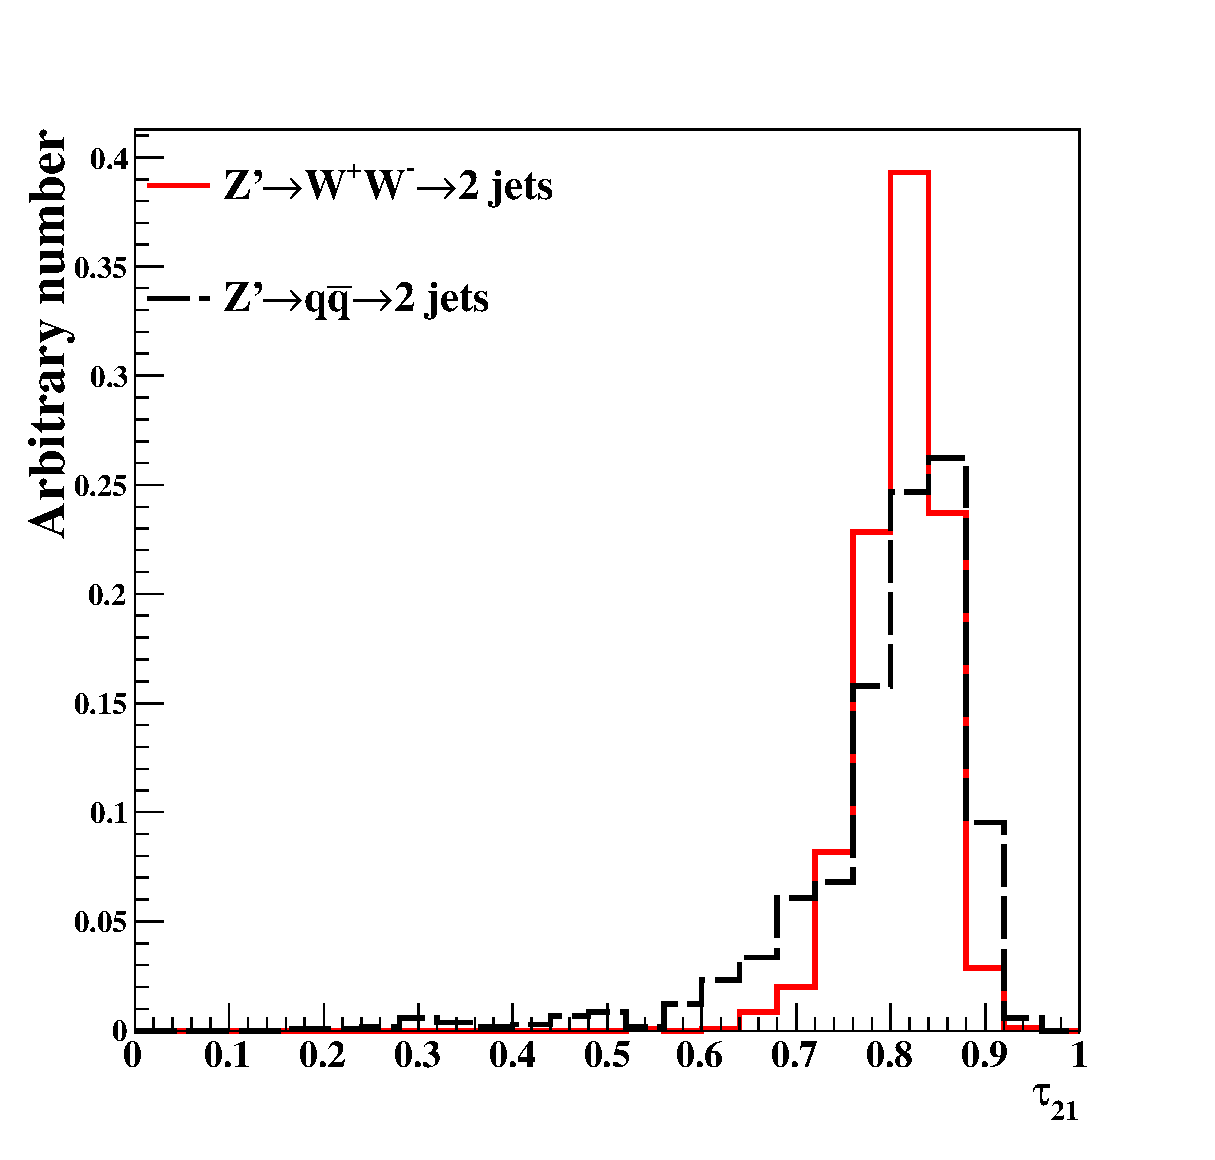
\includegraphics[width=0.3\textwidth]{h_Tau_C/Dis_Rawhit_05GeV_010_tau21_20tev_04_after_cut_Man_25_no_UOF_new_75pa_for_paper.eps}
   }
   \subfigure[5~$\times$~5 cm$^2$] {
   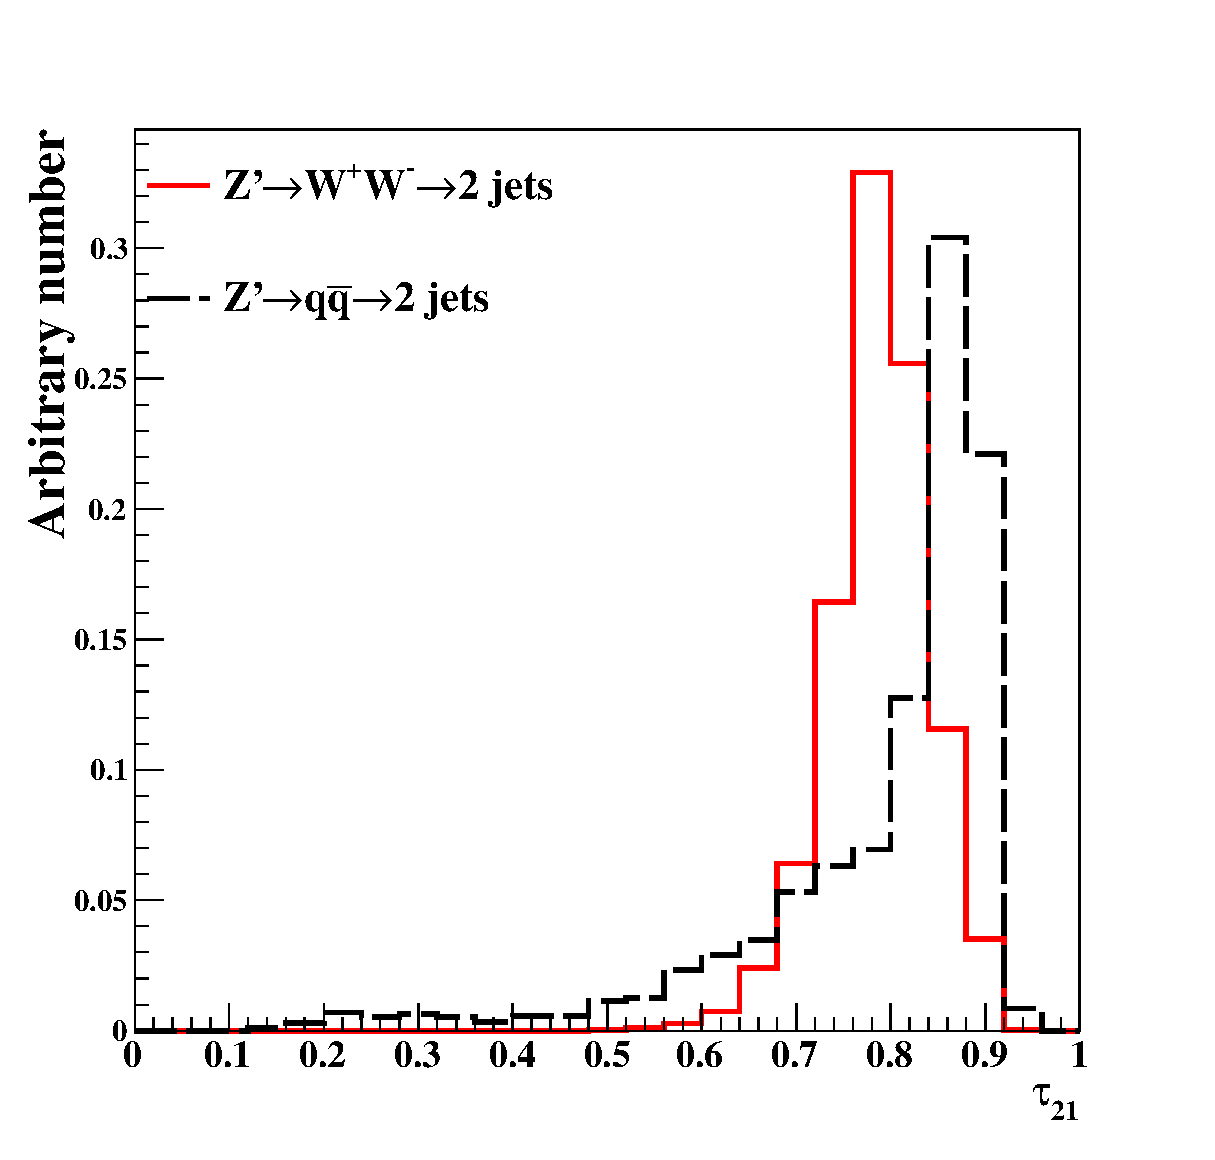
\includegraphics[width=0.3\textwidth]{h_Tau_C/Dis_Rawhit_05GeV_009_tau21_20tev_04_after_cut_Man_25_no_UOF_new_75pa_for_paper.eps}
   }
   \subfigure[1~$\times$~1 cm$^2$] {
   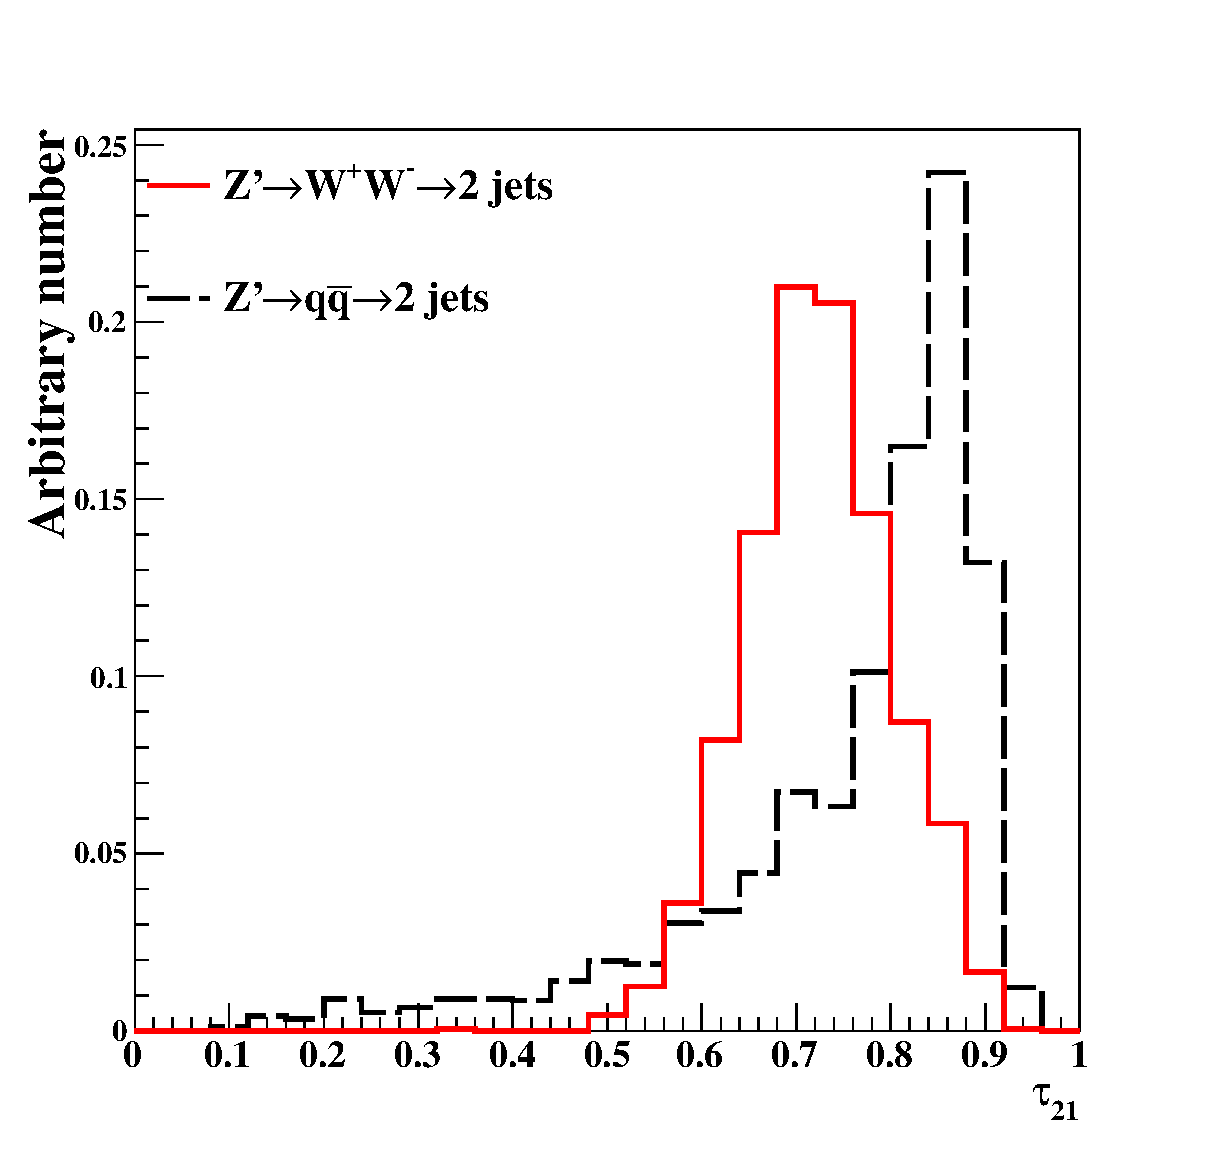
\includegraphics[width=0.3\textwidth]{h_Tau_C/Dis_Rawhit_05GeV_012_tau21_20tev_04_after_cut_Man_25_no_UOF_new_75pa_for_paper.eps}
   }
\end{center}
\caption{Distributions of $\tau_{21}$ for $M(Z') = 20$~TeV for different 
detector granularities. Cell sizes of 20~$\times$~20, 5~$\times$~5, and 1~$\times$~1~cm$^2$ 
are shown here. \label{fig:Rawhit_05GeV_tau21_Dis}}
\end{figure}

\begin{figure}
\begin{center}
   \subfigure[$M(Z')=5$~TeV] {
   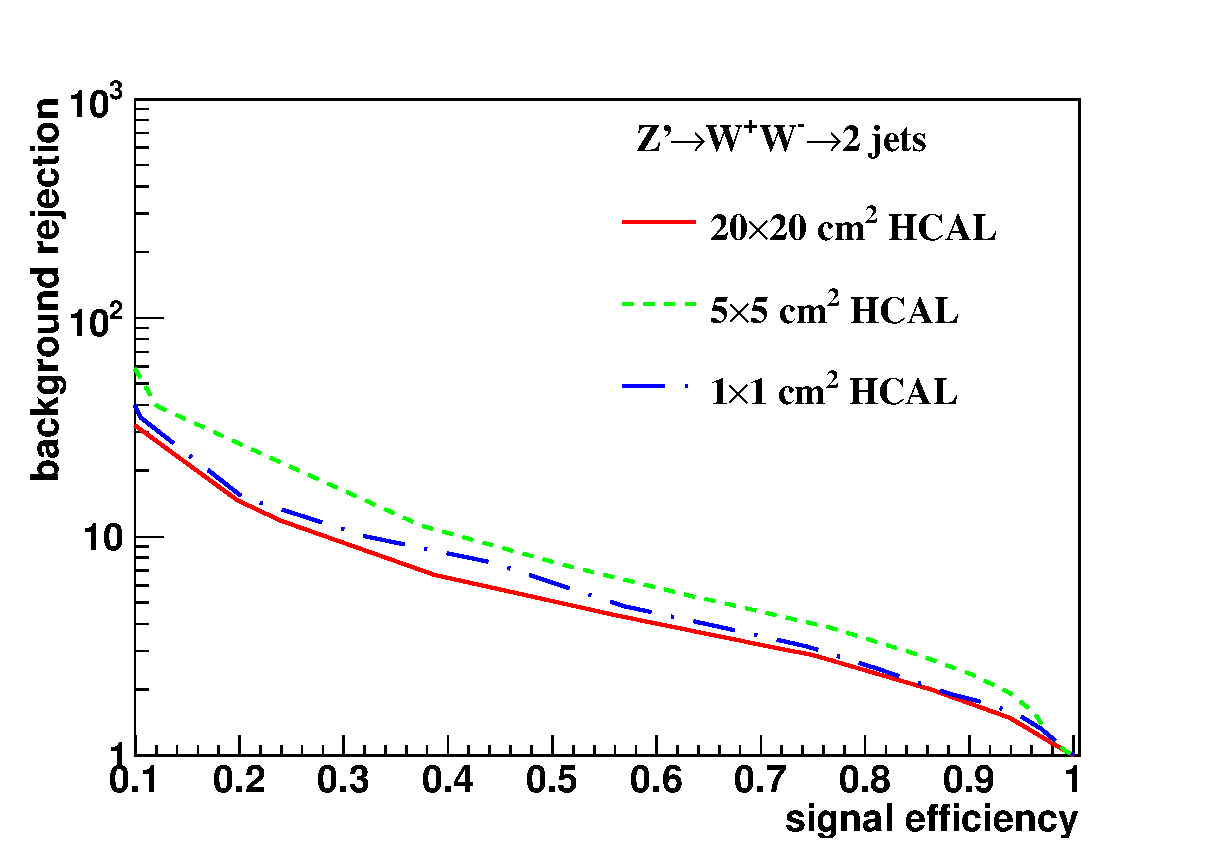
\includegraphics[width=0.43\textwidth]{ROC_Tau_C/Rawhit_05GeV_tau21_5tev_eff_1_New2_after_cut_25bins_no_UOF_new_75pa.eps}
   }
   \subfigure[$M(Z')=10$~TeV] {
   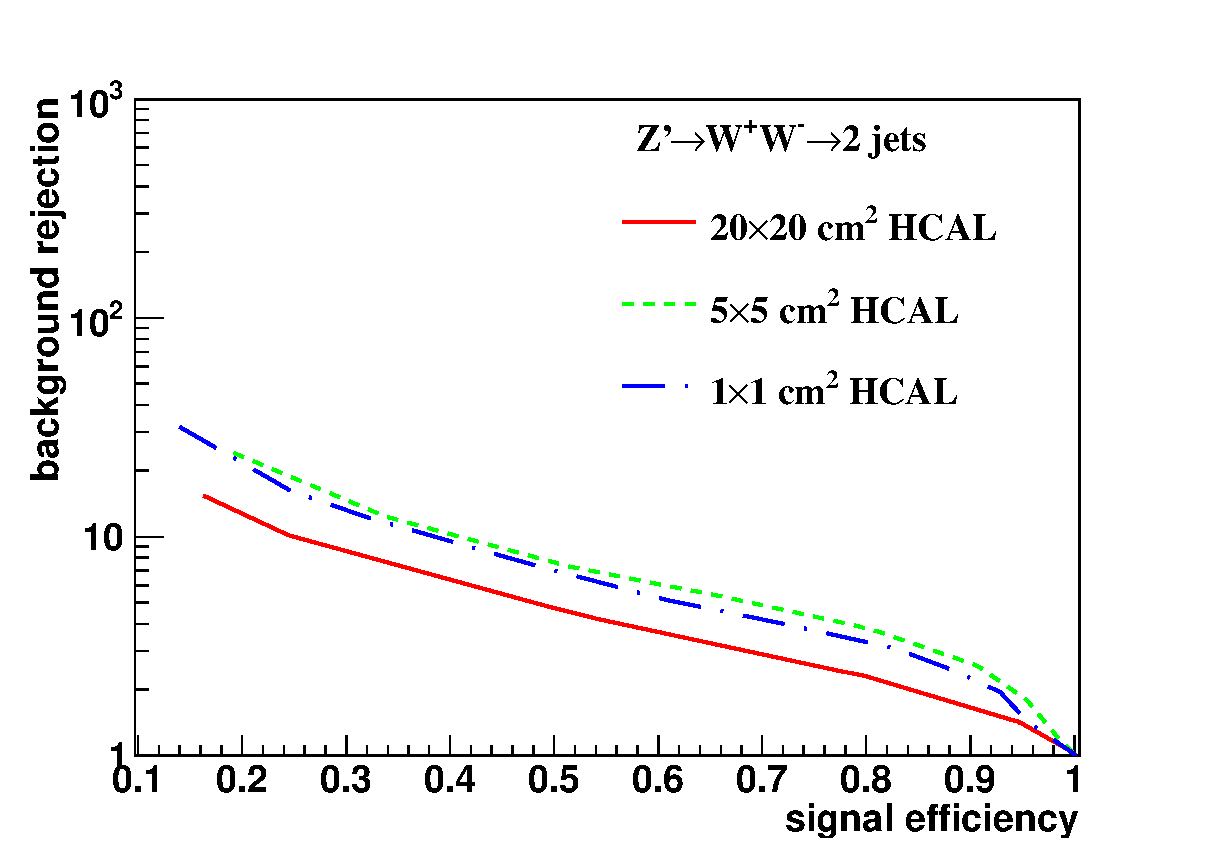
\includegraphics[width=0.43\textwidth]{ROC_Tau_C/Rawhit_05GeV_tau21_10tev_eff_1_New2_after_cut_25bins_no_UOF_new_75pa.eps}
   }
   \subfigure[$M(Z')=20$~TeV] {
   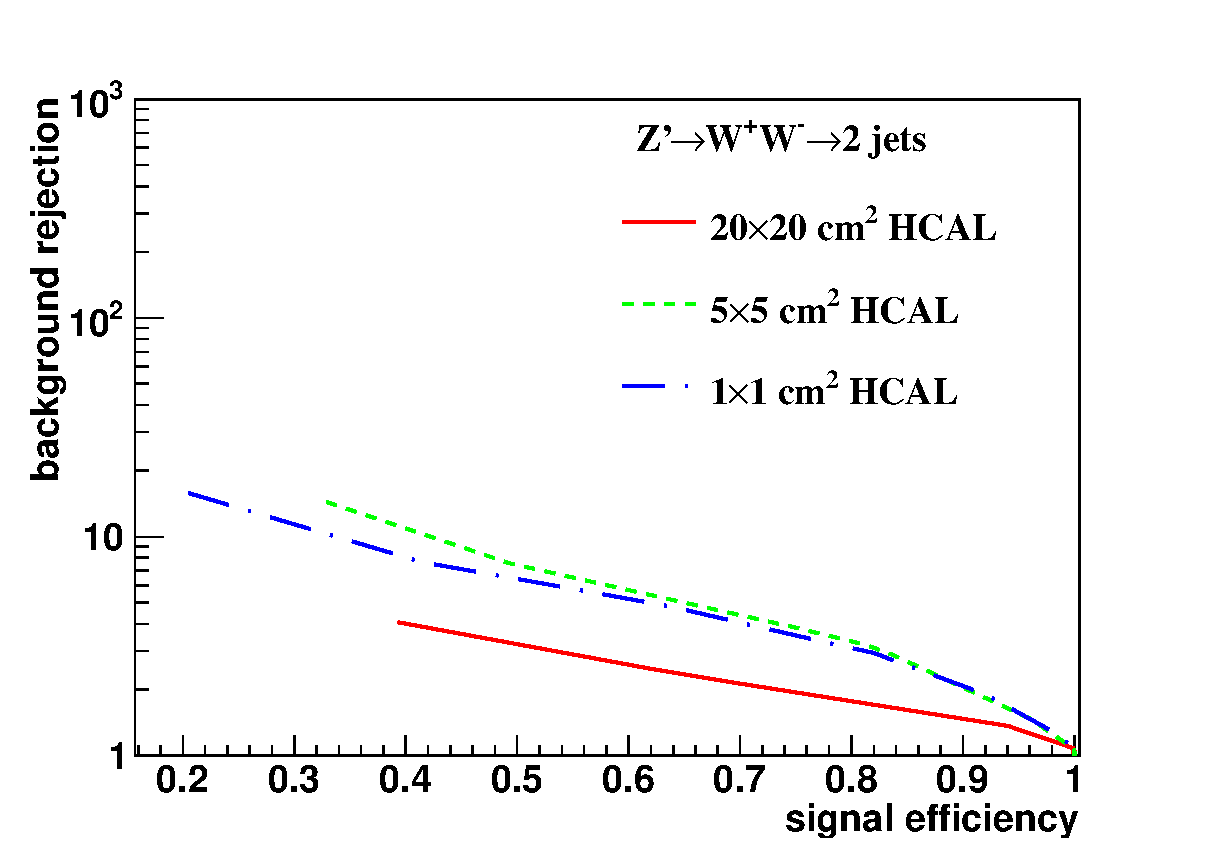
\includegraphics[width=0.43\textwidth]{ROC_Tau_C/Rawhit_05GeV_tau21_20tev_eff_1_New2_after_cut_25bins_no_UOF_new_75pa.eps}
   }
   \subfigure[$M(Z')=40$~TeV] {
   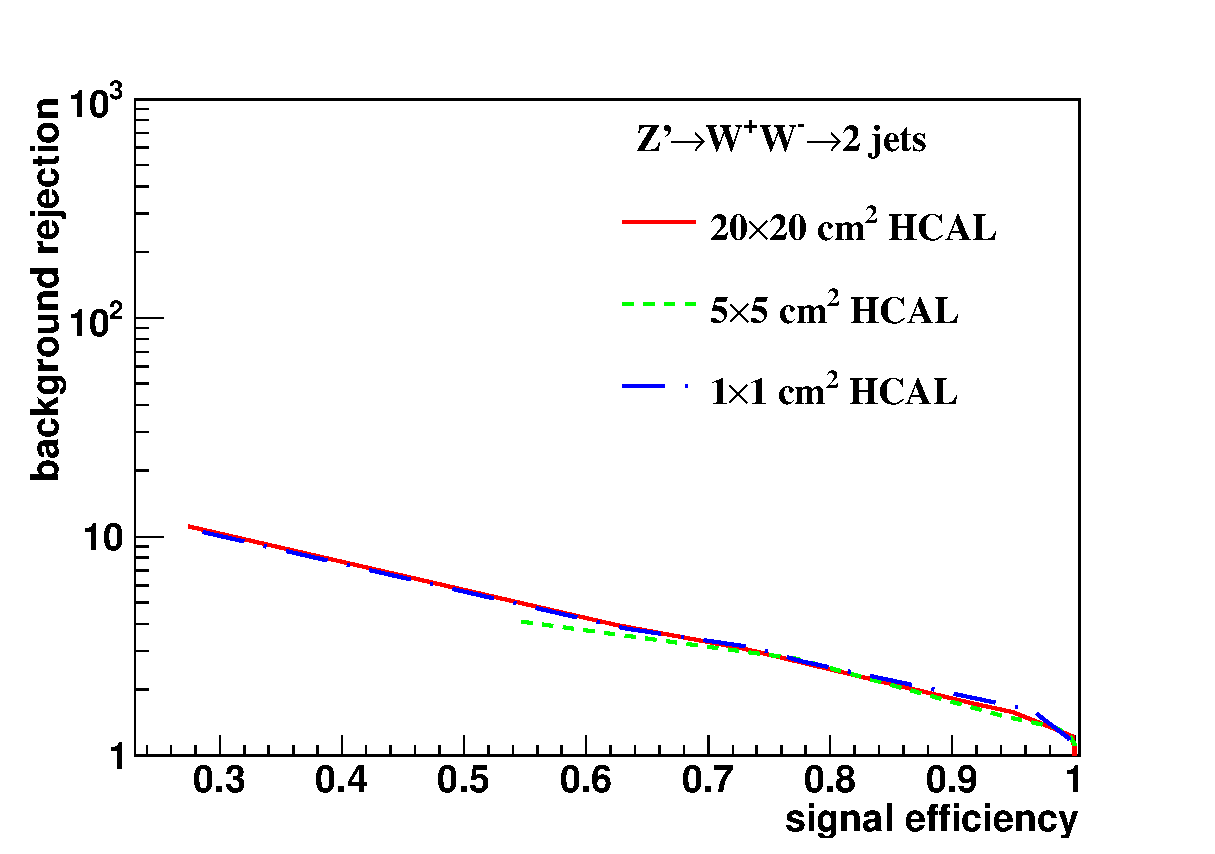
\includegraphics[width=0.43\textwidth]{ROC_Tau_C/Rawhit_05GeV_tau21_40tev_eff_1_New2_after_cut_25bins_no_UOF_new_75pa.eps}
   }
\end{center}
\caption{Signal efficiency versus background rejection rate using $\tau_{21}$.
Resonance masses of (a) 5~TeV, (b) 10~TeV, (c) 20~TeV and (d) 40~TeV are shown 
here. 
In each figure, the three ROC curves correspond to different cell sizes.
\label{fig:Rawhit_05GeV_tau21_ROC}
}
\end{figure}

With this {\it a-priori} mass window pre-selection, the signal and background efficiencies of 
various $\tau_{21}$ and $\tau_{32}$ window cuts are scanned. 
Since some of the background distributions have long tails and leak into the 
signal-dominated region, we use the following method based on the 
Neyman-Pearson lemma to determine the $\tau$ windows. 
First, we take the ratio of the signal to background $\tau_{21}$ (or $\tau_{32}$) 
histograms. The window is initialized by the bin with the maximum signal to 
background ratio (S/N).  
%$x_\mathrm{low}^\mathrm{seedbin} < \tau_{21} <  x_\mathrm{high}^\mathrm{seedbin}$. 
Comparing the adjacent bins,  the bin with the larger S/N is included  to extend the $\tau_{21}$ (or $\tau_{32}$) 
selection window iteratively.  Every window has its corresponding $\epsilon_\mathrm{sig}$ and 
1/$\epsilon_\mathrm{bkg}$ and an ROC curve is mapped out. 

%In addition to the ROC curves, we use the so-called ``Mann-Whitney'' test~\cite{mann1947} to quantify the detector performance.  The value of the Mann-Whitney $U$ variable is related to the area under the ROC curve; if the $U$ value is bigger, it indicates the signal and background  distributions have similar shapes and cannot be well-separated from  each other. Vice versa, if the $U$ value is smaller, we can achieve better signal and background separation. 

\textcolor{red}{The display for ROC curves and histograms are the same as those shown in Sect.\ref{Rebin_section}, we show the bigger bin width for presenting the histograms, and use the finer bin width to do the analysis.} Figures~\ref{fig:Rawhit_05GeV_tau21_Dis} and~\ref{fig:Rawhit_05GeV_tau32_Dis} 
show the distributions of $\tau_{21}$ and $\tau_{32}$ for $M(Z')=20$~TeV 
after applying the requirement on the soft drop mass. The signals considered are 
the $Z'\rightarrow WW$ (for $\tau_{21}$) and 
$Z' \rightarrow t\bar{t}$ (for $\tau_{32}$) processes. 
Figures~\ref{fig:Rawhit_05GeV_tau21_ROC} and~\ref{fig:Rawhit_05GeV_tau32_ROC} 
present the ROC curves from different detector cell sizes and resonance masses, 
respectively. We find that the performance of the $1\times1~\mathrm{cm}^2$ and $5\times5~\mathrm{cm}^2$ cell sizes is similar for both the $ \tau_{21} $ and the $ \tau_{32} $ variables, for
 all resonance masses in the 5-40~TeV range. These smaller cell sizes yield a higher performance than 
 the $20\times20~\mathrm{cm}^2$ cell size when using the $ \tau_{21} $ variable, for resonance masses of 5, 10 and 20 TeV in the $WW$ final state. In the case of the $ \tau_{32} $ variable, 
  the results are ambiguous, as the $20\times20~\mathrm{cm}^2$ cell size is more (less) performant for low (high) efficiency selection criteria. 

%Figure~\ref{fig:Rawhit_05GeV_total_Mann} presents the summary plots of $\tau_{21}$ and $\tau_{32}$ with various detector cell sizes and resonance masses using the Mann-Whitney test.  For $\tau_{21}$ the detector performance improves when cell size is reduced from $20\times20~\mathrm{cm}^2$ to $5\times5~\mathrm{cm}^2$ for all resonance masses.  However, when the cell size  is reduced further to $1\times1~\mathrm{cm}^2$, the results are ambiguous and depend on the resonance mass. In the case of $\tau_{32}$, there is a smaller improvement from $20\times20~\mathrm{cm}^2$ to $5\times5~\mathrm{cm}^2$ cell size (as compared to $\tau_{21}$), and further improvement with   $1\times1~\mathrm{cm}^2$ cell size is not significant. 

\subsection{Energy correlation function \label{sec:ecf}}
The energy correlation function (ECF)~\cite{Larkoski:2013eya} is defined as follows: 
%\begin{equation} \label{eq:ECF_Original}
%ECF(N,\beta)=\sum_{i_{1}<i_{2}<....<i_{N}\in J} (\prod_{a=1}^{N}E_{ia})(\prod_{%b=1}^{N-1}\prod_{c=b+1}^{N} \theta_{i_{b}i_{c}})^{\beta}, 
%\end{equation}
\begin{equation} \label{eq:ECF_Modified}
ECF(N,\beta)=\sum_{i_{1}<i_{2}<....<i_{N}\in J} \left(\prod_{a=1}^{N}p_{\mathrm{T}ia}\right)\left(\prod_{b=1}^{N-1}\prod_{c=b+1}^{N} R_{i_{b}i_{c}}\right)^{\beta},
\end{equation}
where the sum is over all constituents in jet $J$, $\pt$ is the transverse 
momentum of each constituent, and $R_{mn}$ is the distance between two constituents $m$ and $n$ in the $y$-$\phi$ plane.  
In order to use a dimensionless variable, a parameter $r_{N}$ is defined:
\begin{equation} \label{eq:ECF_ratio}
r_{N}^{(\beta)}\equiv\frac{ECF(N+1,\beta)}{ECF(N,\beta)}.
\end{equation}

%%%%%%%%%% Tau32
%25bins
\begin{figure}
\begin{center}
   \subfigure[20$\times$20 cm$^2$] {
   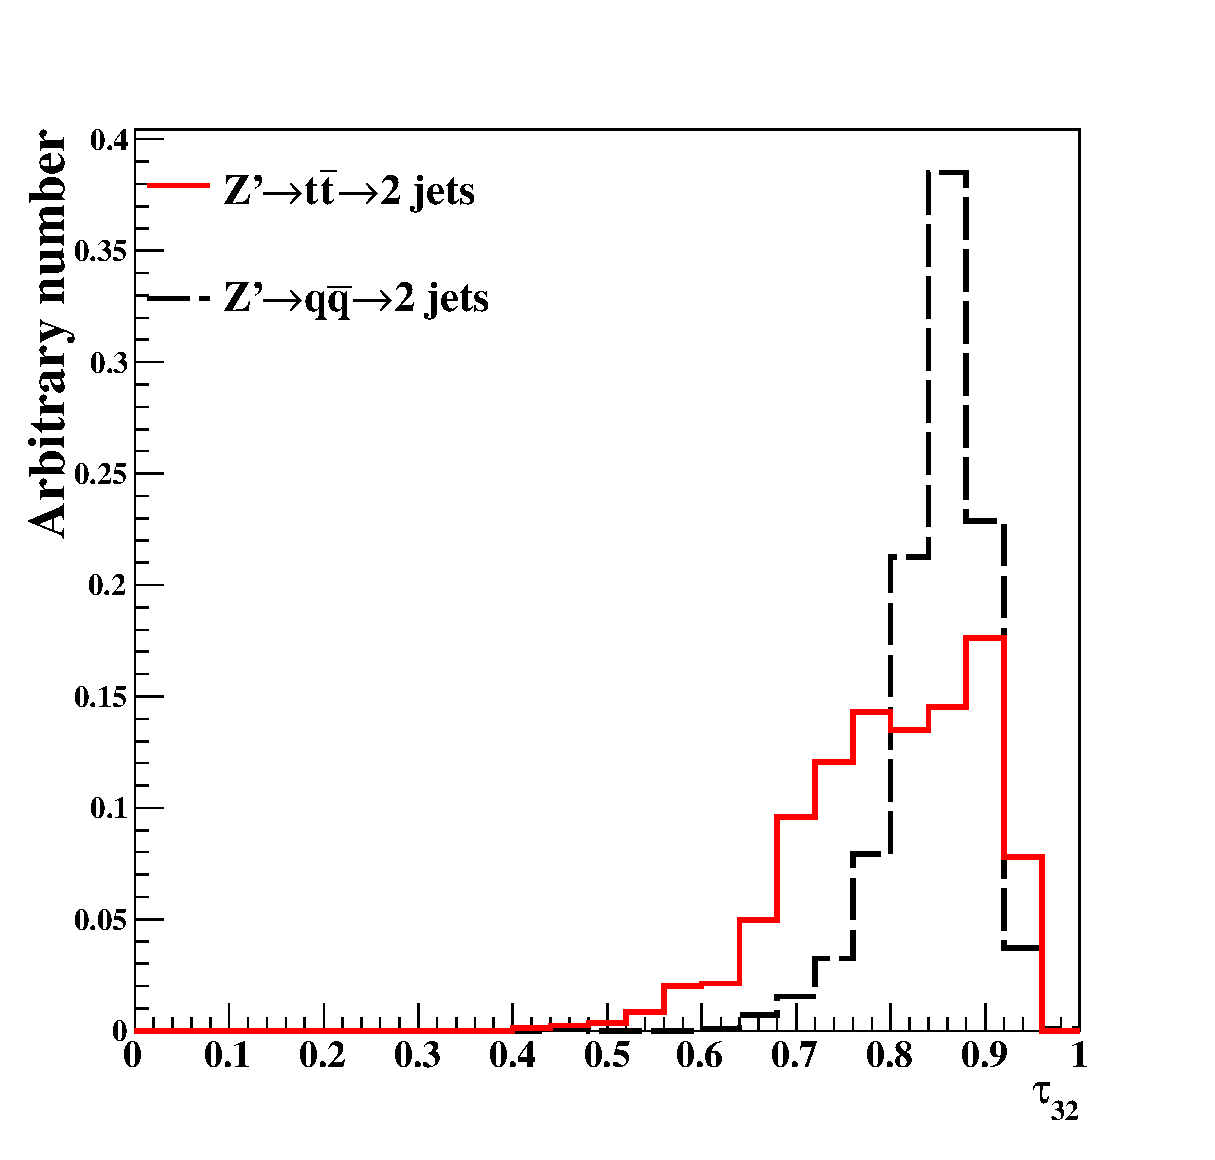
\includegraphics[width=0.3\textwidth]{h_Tau_C/Dis_Rawhit_05GeV_010_tau32_20tev_04_after_cut_Man_25_no_UOF_new_75pa_for_paper.eps}
   }
   \subfigure[5$\times$5 cm$^2$] {
   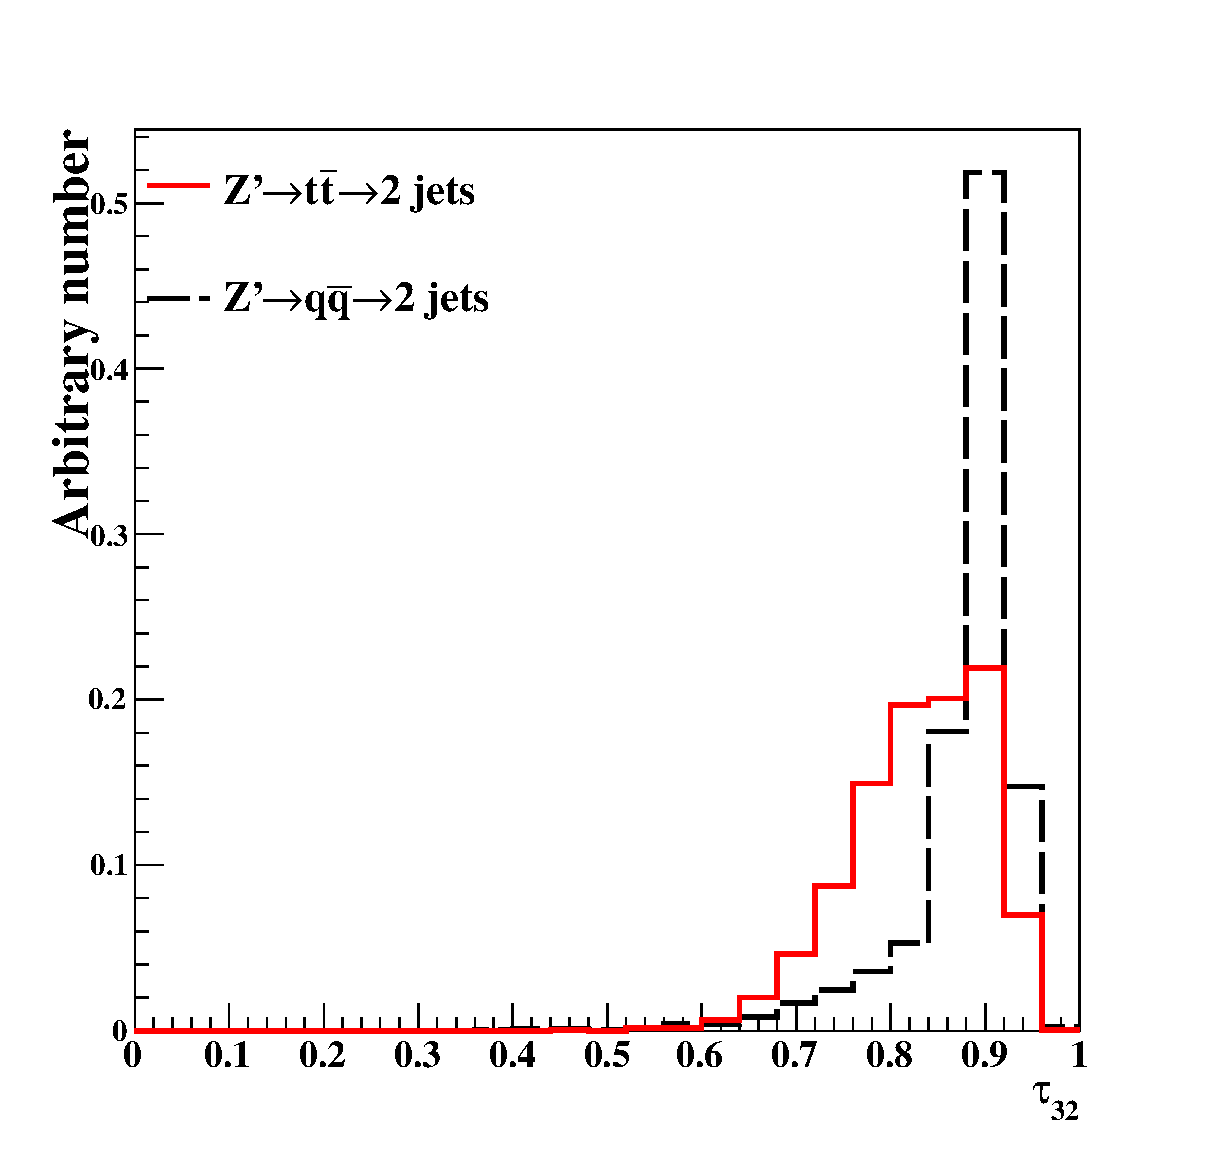
\includegraphics[width=0.3\textwidth]{h_Tau_C/Dis_Rawhit_05GeV_009_tau32_20tev_04_after_cut_Man_25_no_UOF_new_75pa_for_paper.eps}
   }
   \subfigure[1$\times$1 cm$^2$] {
   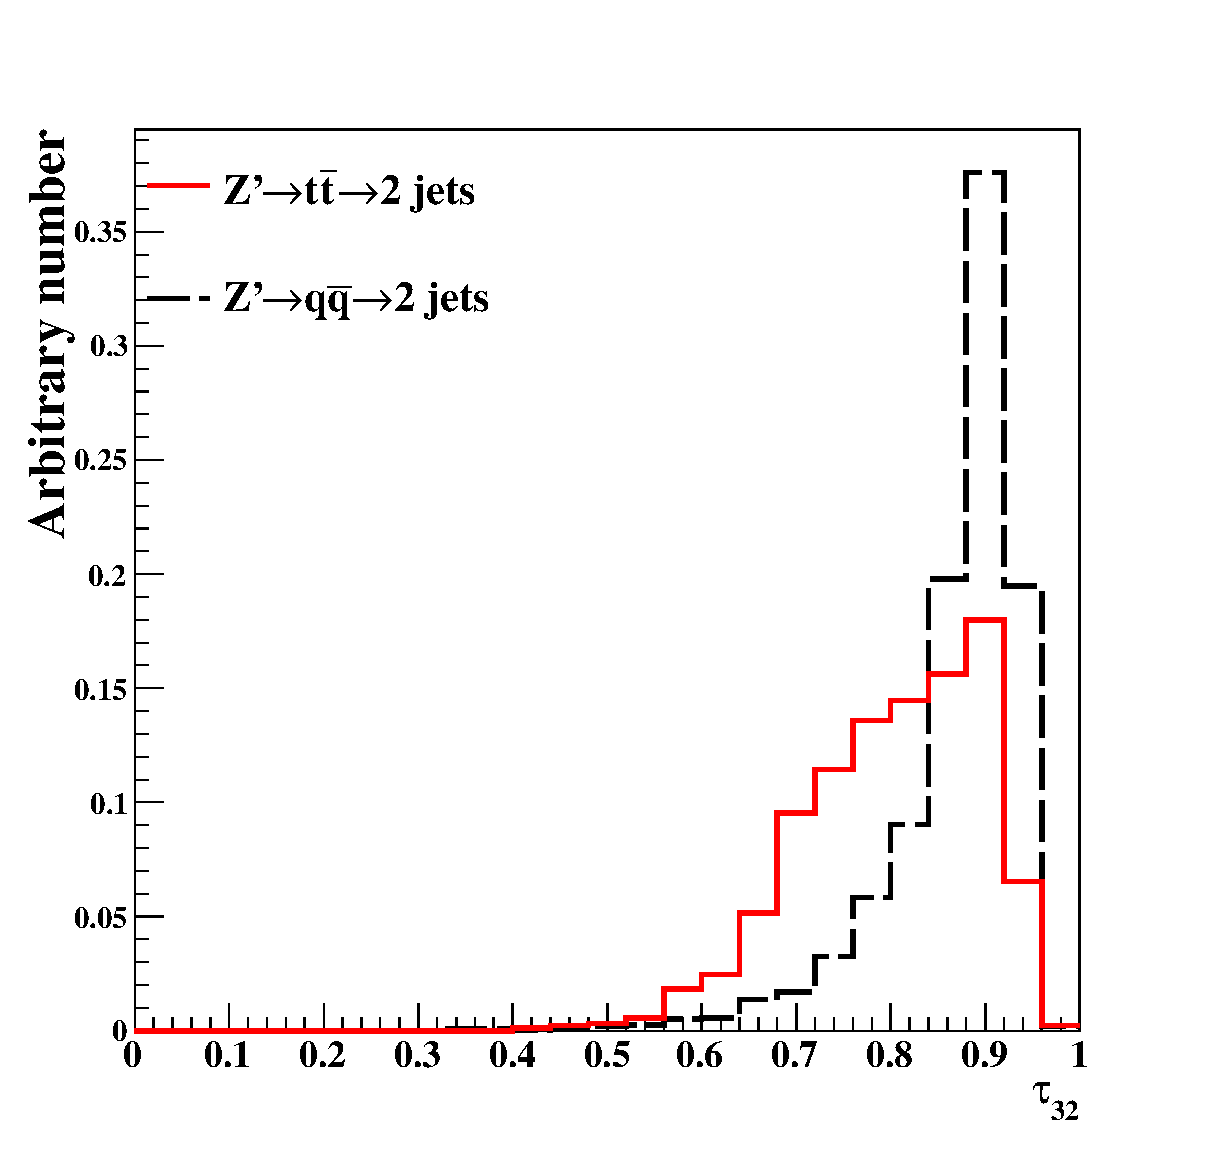
\includegraphics[width=0.3\textwidth]{h_Tau_C/Dis_Rawhit_05GeV_012_tau32_20tev_04_after_cut_Man_25_no_UOF_new_75pa_for_paper.eps}
   }
\end{center}
\caption{Distributions of $\tau_{32}$ for $M (Z') =20$~TeV for different 
detector granularities. Cell sizes of 20~$\times$~20, 5~$\times$~5, and 1~$\times$~1~cm$^2$ 
are shown here.
\label{fig:Rawhit_05GeV_tau32_Dis}
}
\end{figure}

\begin{figure}
\begin{center}
   \subfigure[$M(Z') = 5$~TeV] {
   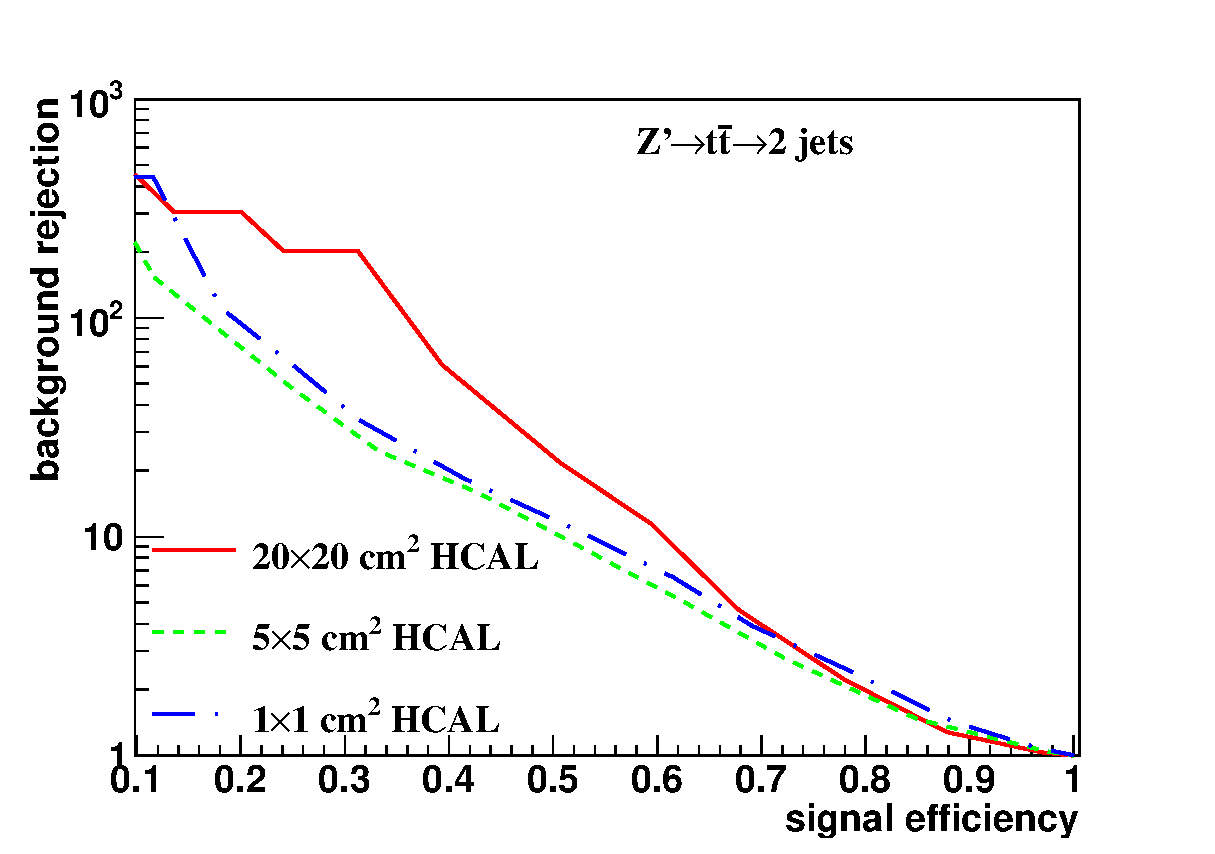
\includegraphics[width=0.43\textwidth]{ROC_Tau_C/Rawhit_05GeV_tau32_5tev_eff_1_New2_after_cut_25bins_no_UOF_new_75pa.eps}\hfill
   }
   \subfigure[$M(Z')=10$~TeV] {
   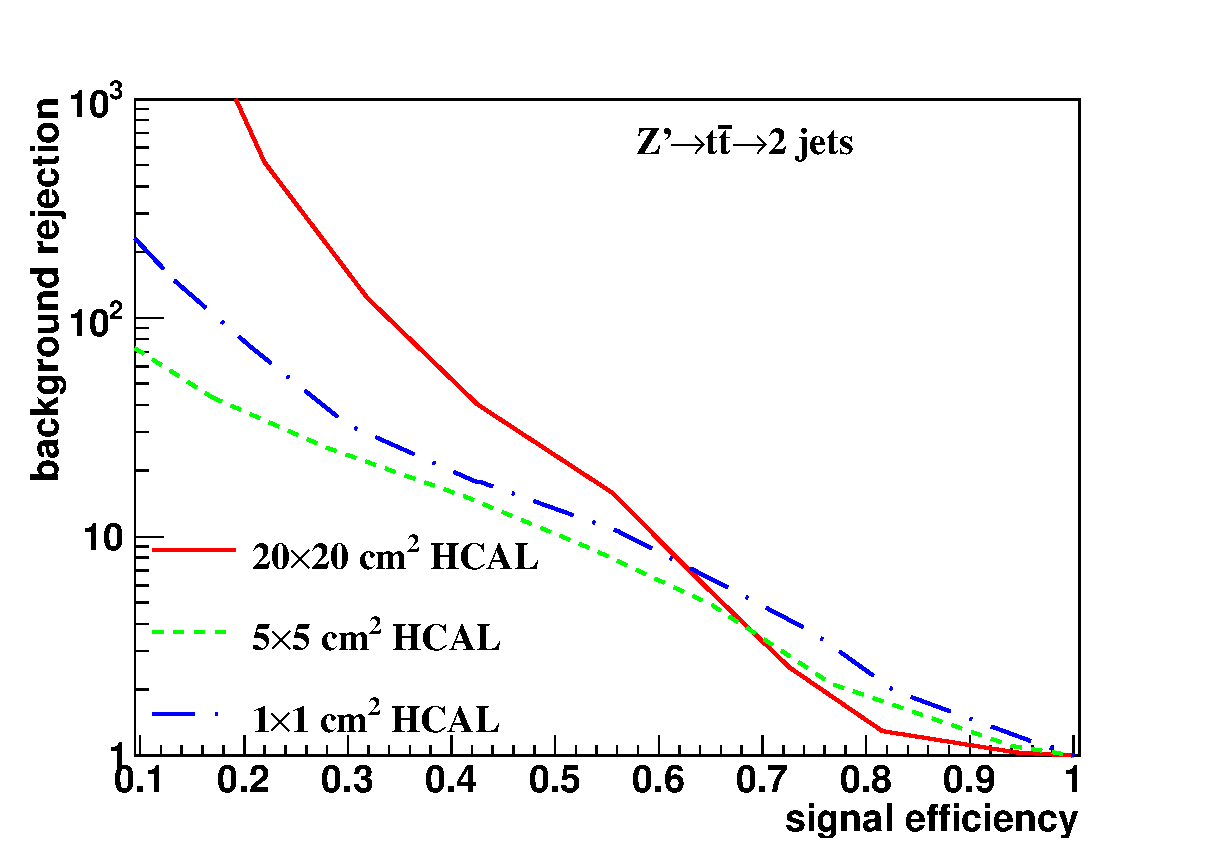
\includegraphics[width=0.43\textwidth]{ROC_Tau_C/Rawhit_05GeV_tau32_10tev_eff_1_New2_after_cut_25bins_no_UOF_new_75pa.eps}
   }
   \subfigure[$M(Z')=20$~TeV] {
   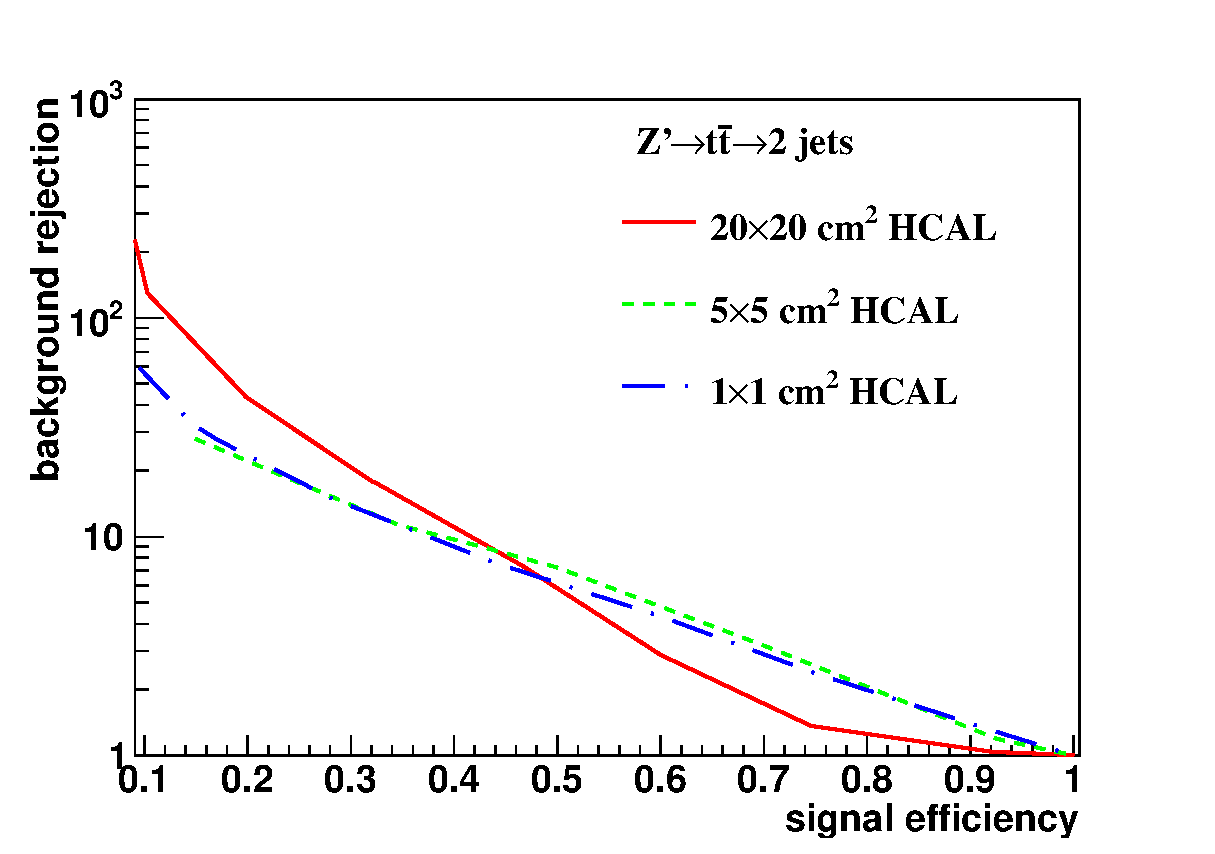
\includegraphics[width=0.43\textwidth]{ROC_Tau_C/Rawhit_05GeV_tau32_20tev_eff_1_New2_after_cut_25bins_no_UOF_new_75pa.eps}
   }
   \subfigure[$M(Z')=40$~TeV] {
   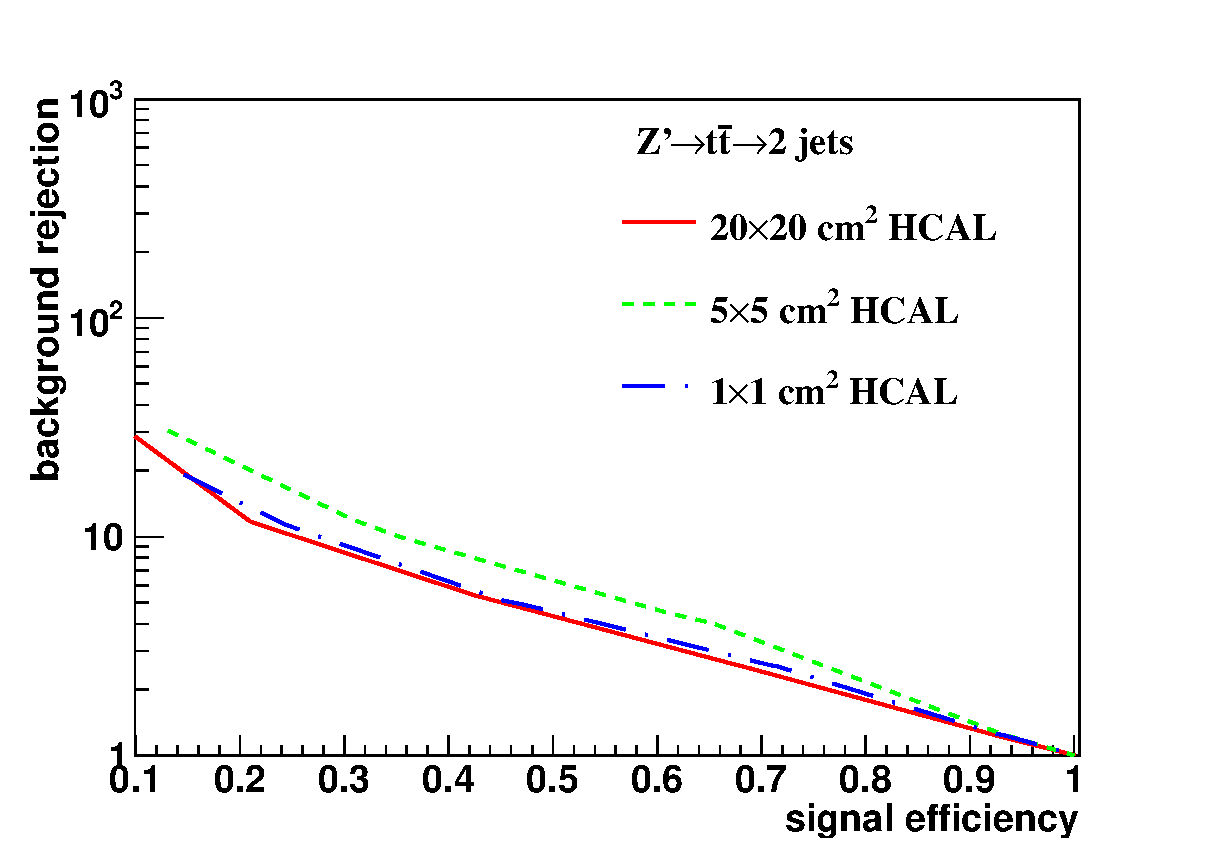
\includegraphics[width=0.43\textwidth]{ROC_Tau_C/Rawhit_05GeV_tau32_40tev_eff_1_New2_after_cut_25bins_no_UOF_new_75pa.eps}
   }
\end{center}
\caption{Signal efficiency versus background rejection rate using $\tau_{32}$. 
Resonance masses of (a) 5~TeV, (b) 10~TeV, (c) 20~TeV and (d) 40~TeV are shown 
here. In each figure, the three ROC curves correspond to different HCAL cell 
sizes.
\label{fig:Rawhit_05GeV_tau32_ROC}
}
\end{figure}


%%%%%%%%%%%%%%% c2b1
%25bins 
\begin{figure}
\centering
\begin{center}
   \subfigure[20~$\times$~20~cm$^2$] {
   \centering
   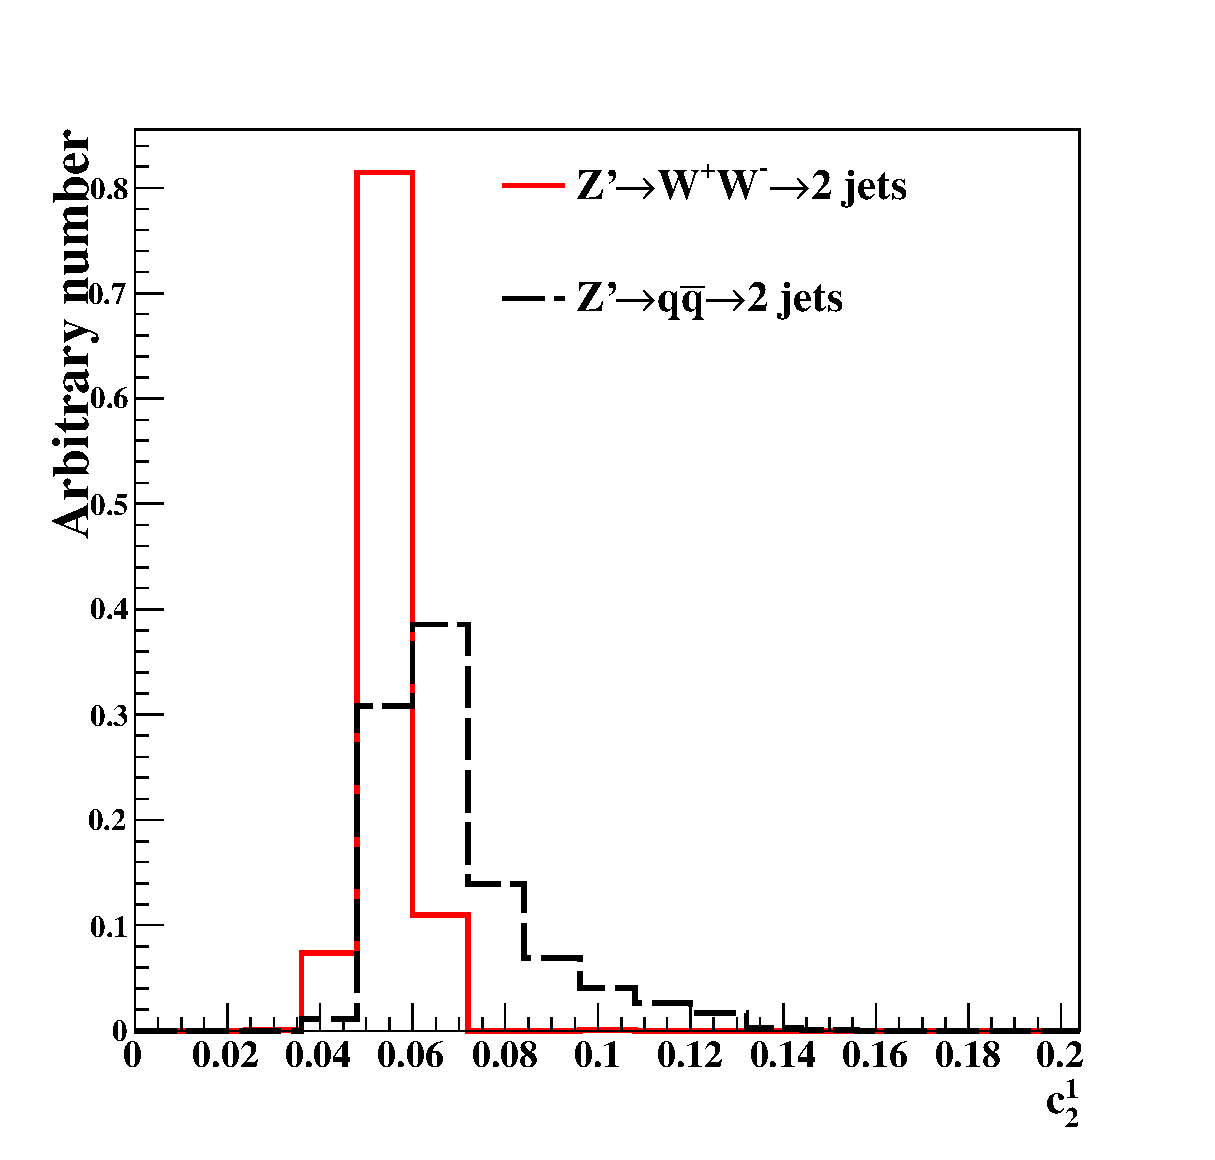
\includegraphics[width=0.3\textwidth]{h_Tau_C/Dis_Rawhit_05GeV_010_c2b1_20tev_04_after_cut_Man_25_no_UOF_new_75pa_for_paper.eps}
   }
   \subfigure[5~$\times$~5~cm$^2$] {
   \centering
   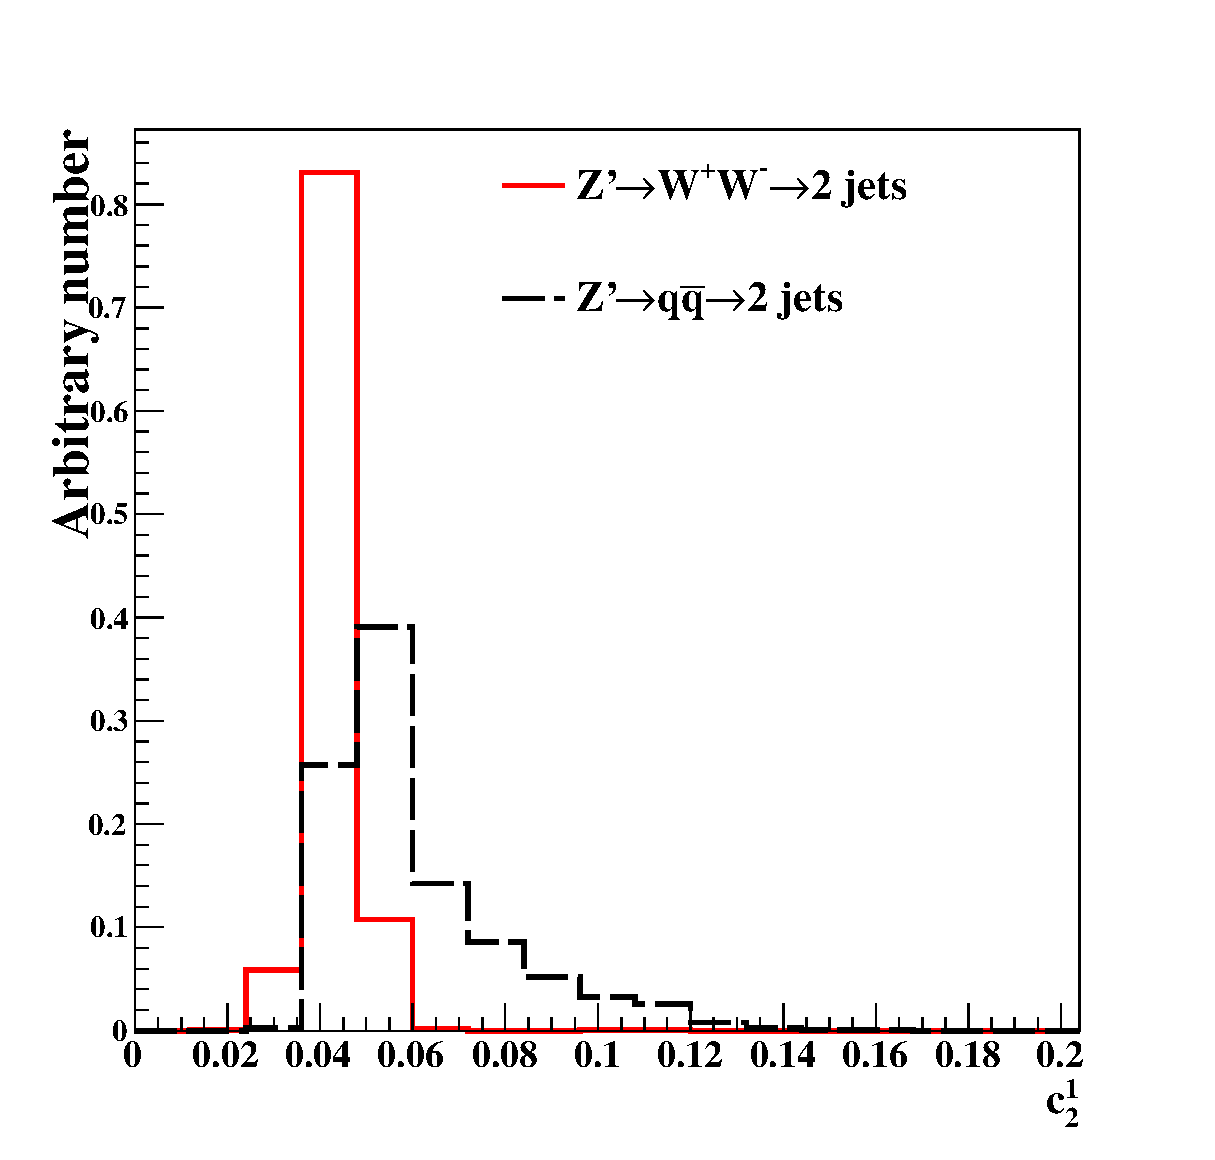
\includegraphics[width=0.3\textwidth]{h_Tau_C/Dis_Rawhit_05GeV_009_c2b1_20tev_04_after_cut_Man_25_no_UOF_new_75pa_for_paper.eps}
   }
   \subfigure[1~$\times$~1~cm$^2$] {
   \centering
   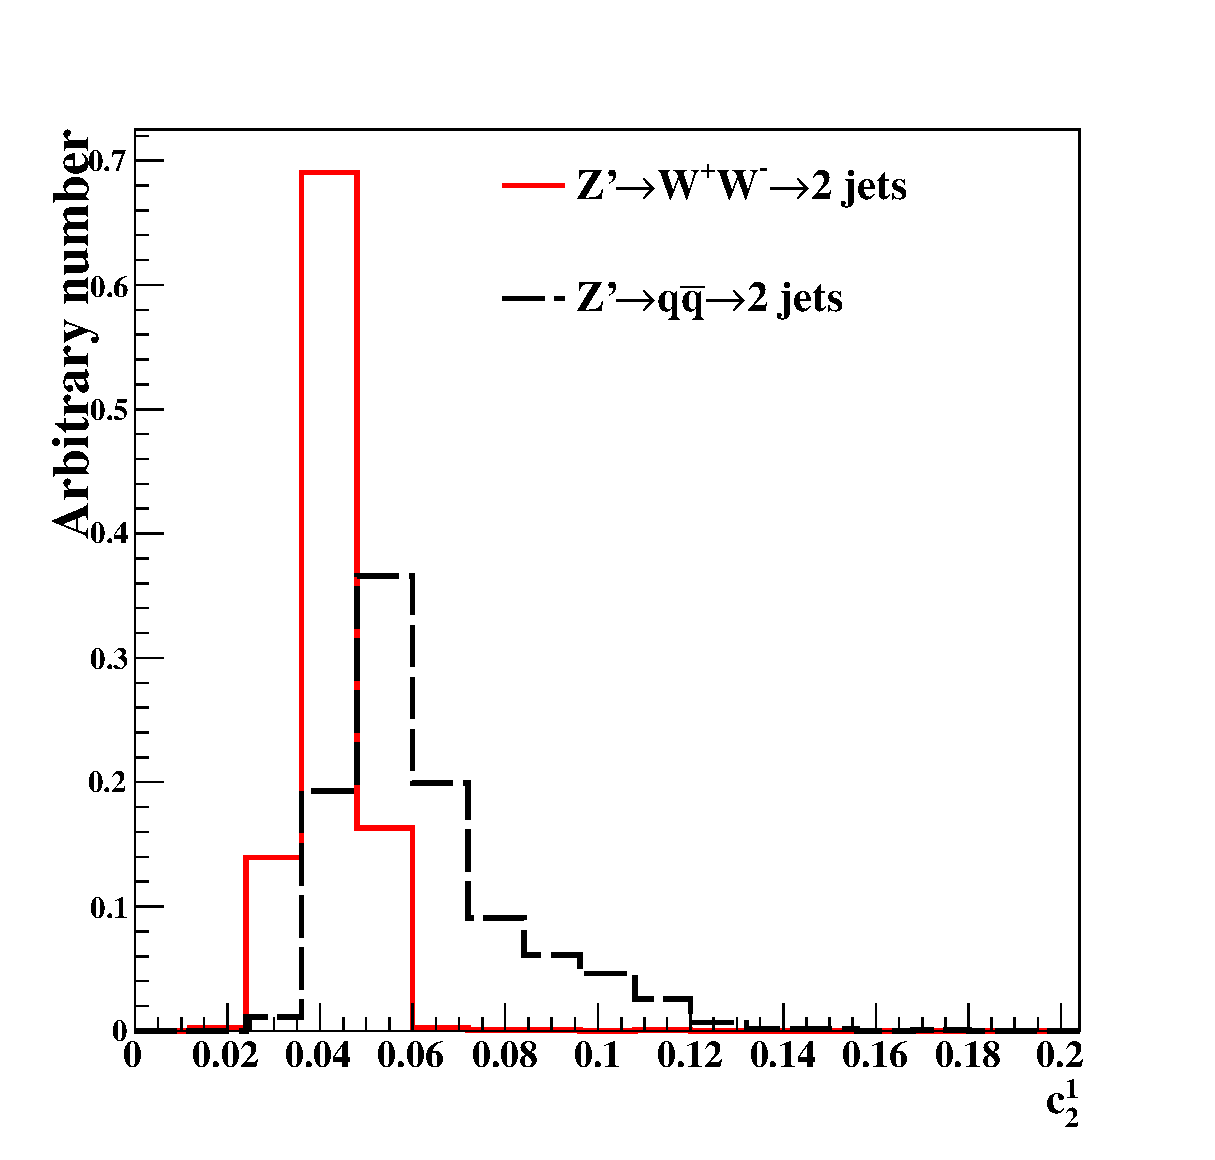
\includegraphics[width=0.3\textwidth]{h_Tau_C/Dis_Rawhit_05GeV_012_c2b1_20tev_04_after_cut_Man_25_no_UOF_new_75pa_for_paper.eps}
   }
\end{center}
\caption{Distributions of $C_2^1$ with $M(Z')= 20$~TeV for different 
detector granularities. Cell sizes of 20~$\times$~20, 5~$\times$~5, and 1~$\times$~1~cm$^2$ 
are shown here.}
\label{fig:Rawhit_05GeV_c2b1_Dis}
\end{figure}

\begin{figure}
\begin{center}
   \subfigure[$M(Z')=5$~TeV] {
   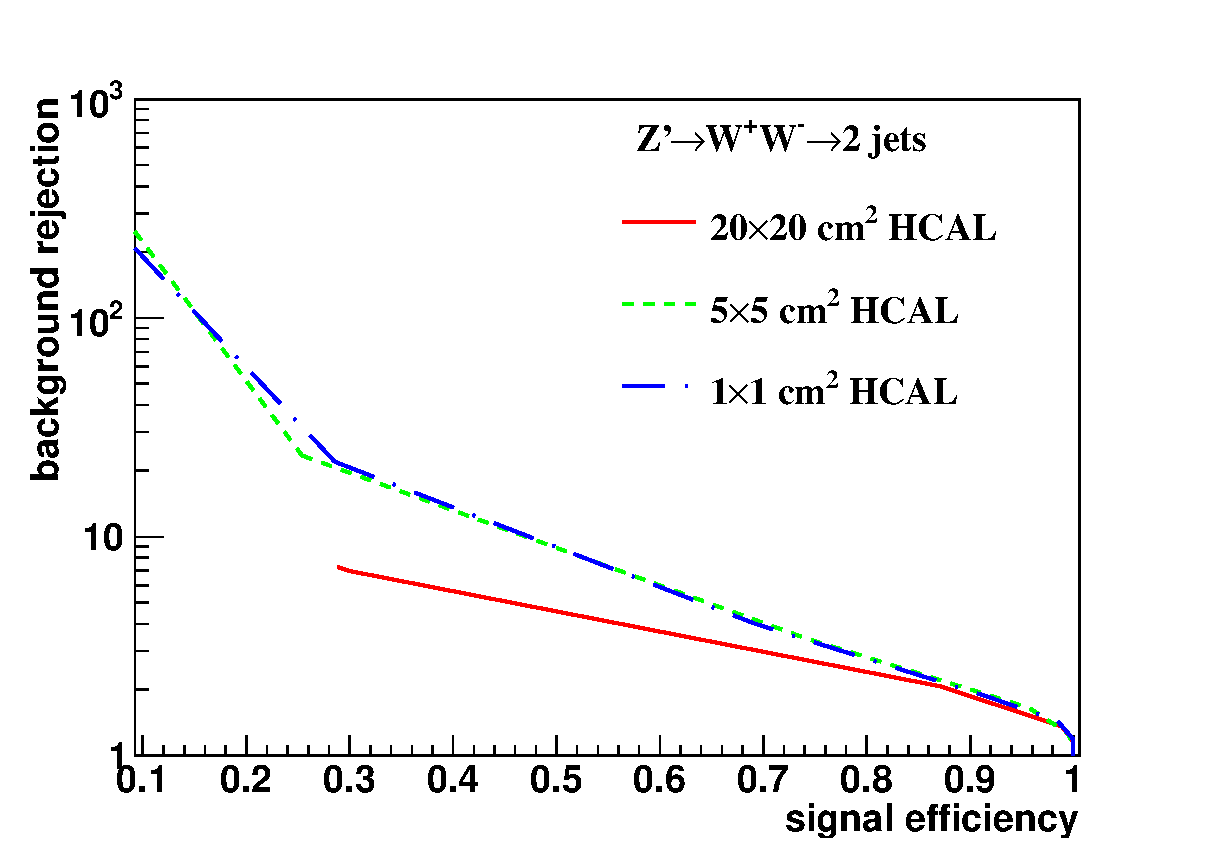
\includegraphics[width=0.43\textwidth]{ROC_Tau_C/Rawhit_05GeV_c2b1_5tev_eff_1_New2_after_cut_25bins_no_UOF_new_75pa.eps}\hfill
   }
   \subfigure[$M(Z')=10$~TeV] {
   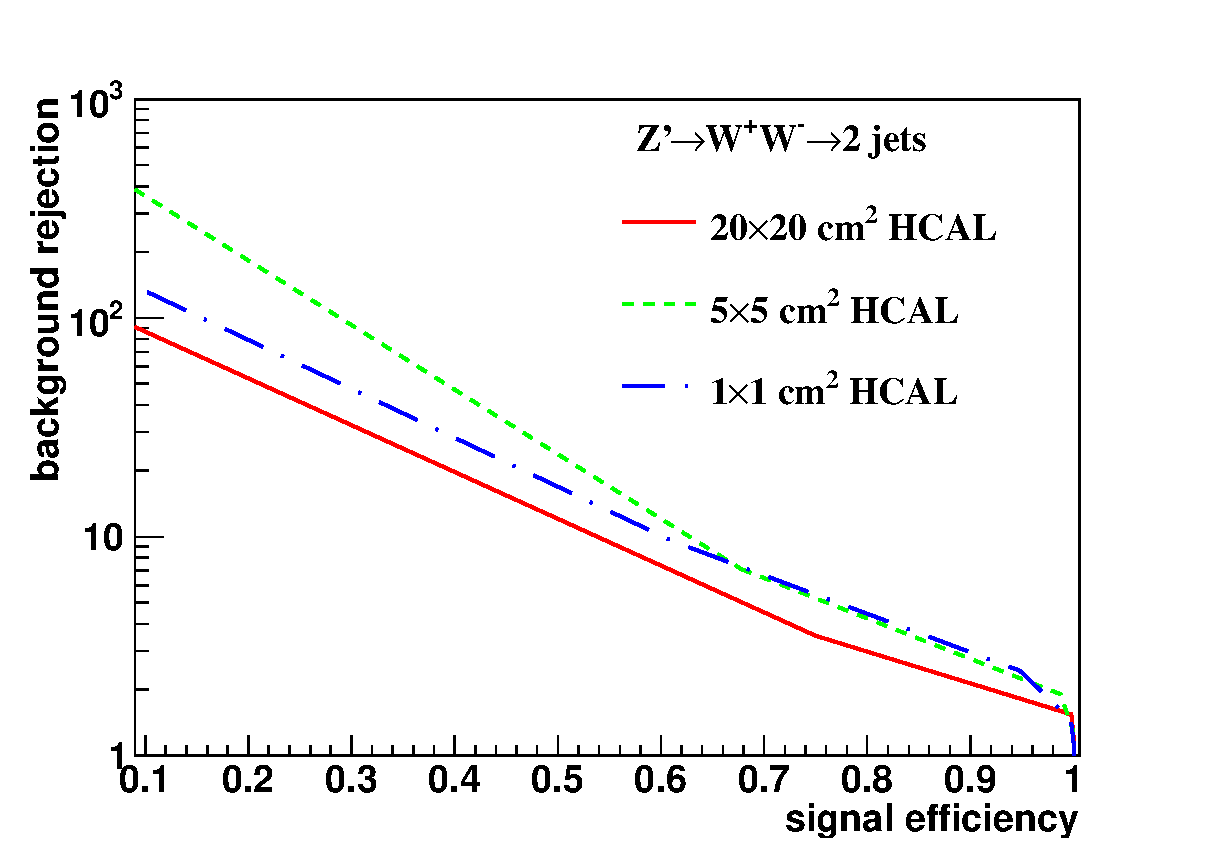
\includegraphics[width=0.43\textwidth]{ROC_Tau_C/Rawhit_05GeV_c2b1_10tev_eff_1_New2_after_cut_25bins_no_UOF_new_75pa.eps}
   }
   \subfigure[$M(Z')=20$~TeV] {
   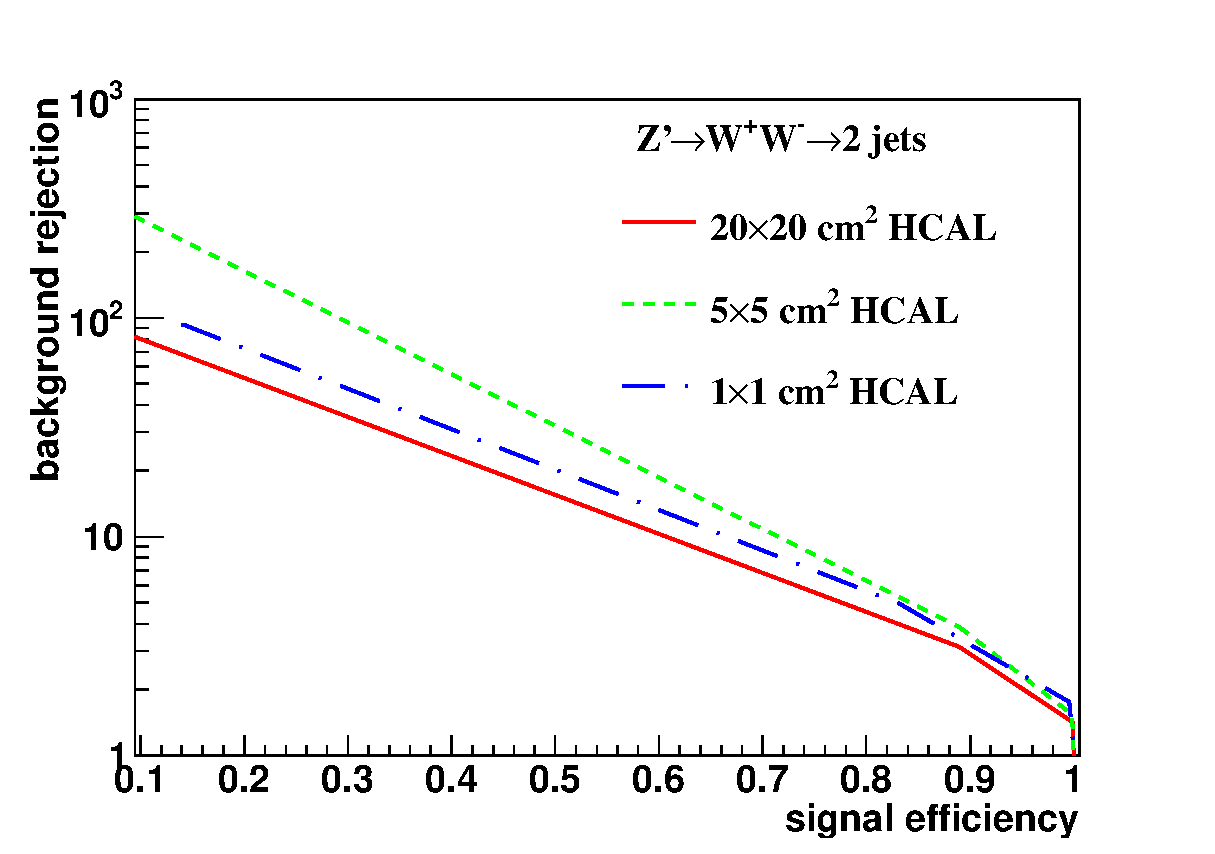
\includegraphics[width=0.43\textwidth]{ROC_Tau_C/Rawhit_05GeV_c2b1_20tev_eff_1_New2_after_cut_25bins_no_UOF_new_75pa.eps}
   }
   \subfigure[$M(Z')=40$~TeV] {
   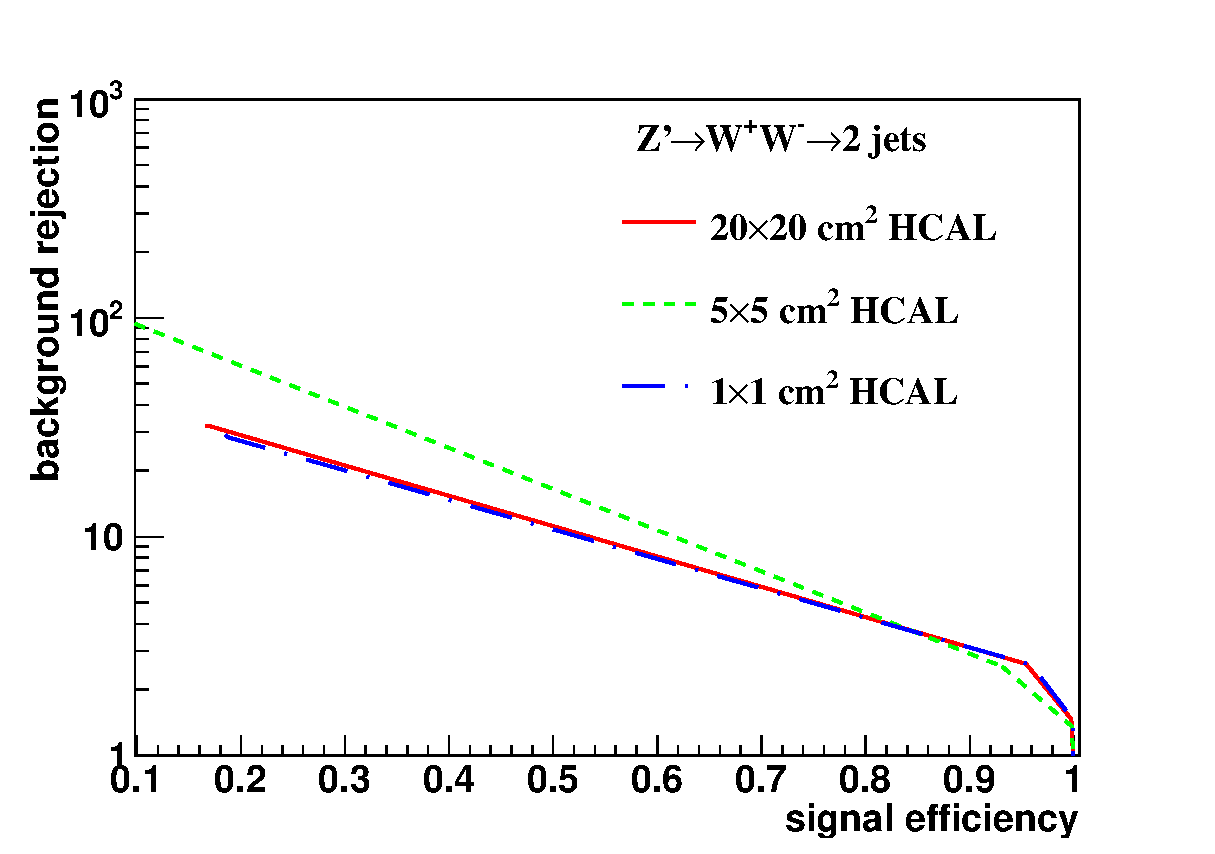
\includegraphics[width=0.43\textwidth]{ROC_Tau_C/Rawhit_05GeV_c2b1_40tev_eff_1_New2_after_cut_25bins_no_UOF_new_75pa.eps}
   }
\end{center}
\caption{Signal efficiency versus background rejection rate using $C_{2}^{1}$. 
The resonance masses of (a) 5~TeV, (b) 10~TeV, (c) 20~TeV, and (d) 40~TeV are shown 
here. In each figure, the three ROC curves correspond to different detector 
sizes.}
\label{fig:Rawhit_05GeV_c2b1_ROC}
\end{figure}



The idea of $r_N$ comes from $N$-subjettiness $\tau_N$. Both $r_N$ and $\tau_N$ 
are linear in the energy of the soft radiation for a system of $N$ partons  accompanied 
by  soft radiation. In general, if the system has $N$ subjets, $ECF(N+1,\beta)$ 
should be significantly smaller than $ECF(N,\beta)$. Therefore, we can use this
 feature to distinguish jets with different numbers  of subjets. 
As in Sect.~\ref{sec:nsub}, the ratio $r_N/r_{N-1}$, denoted by $C_N$, 
(double-ratios of ECFs) is used to study the detector performance: 
\begin{equation}
C_{N}^{(\beta)}\equiv\frac{r_{N}^{(\beta)}}{r_{N-1}^{(\beta)}}=\frac{ECF(N-1,\beta)ECF(N+1,\beta)}{ECF(N,\beta)^2}.
\end{equation}
In our analysis, we set $N=2$ and $\beta=1$ ($C_2^1$).

Figure~\ref{fig:Rawhit_05GeV_c2b1_Dis} presents the histograms of $C_{2}^{1}$ 
with $M(Z')=20$~TeV after making the requirement on the soft drop mass. 
The signal considered is the $Z' \rightarrow WW$ process. 
Figure~\ref{fig:Rawhit_05GeV_c2b1_ROC} shows the ROC curves from different 
detector cell sizes for each resonance mass. One can see that 
the $5 \times 5$~$\mathrm{cm}^2$ cell size improves upon the $20 \times 20$~$\mathrm{cm}^2$ cell size, and either matches or improves upon the $1 \times 1$~$\mathrm{cm}^2$ cell size,
   for all resonance masses. 
%Figure~\ref{fig:Rawhit_05GeV_total_Mann} summarizes the result of  the Mann-Whitney test for $C_{2}^{1}$, which confirms this conclusion. 


\begin{comment}
%25bins Mann-Whitney
\begin{figure}
\begin{center}
   \subfigure[$\tau_{21}$] {
   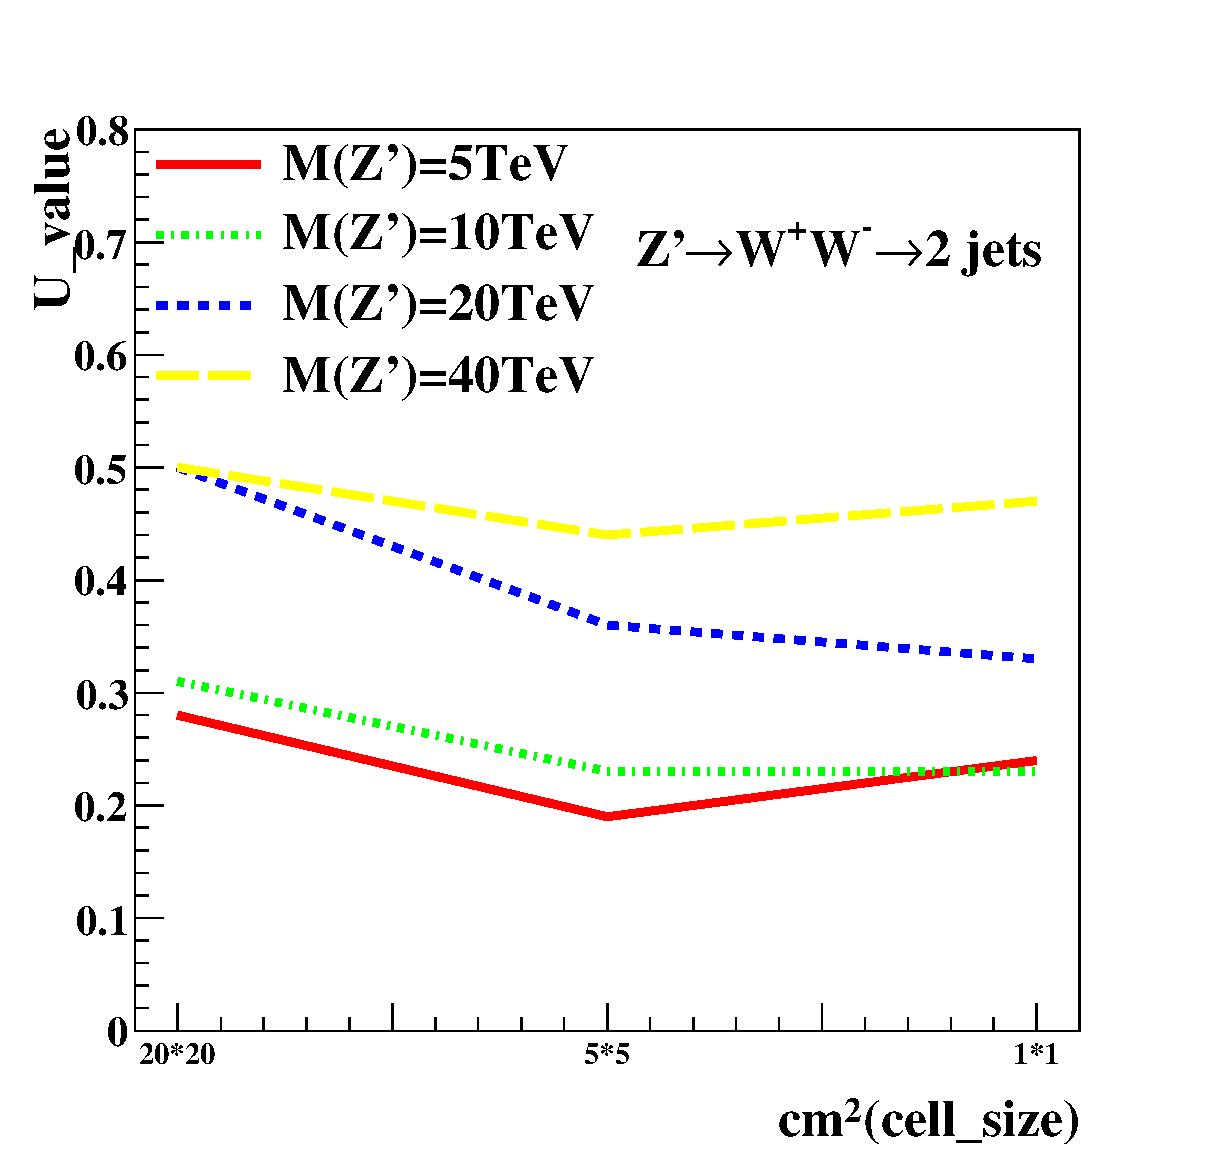
\includegraphics[width=0.3\textwidth]{Mann_Sum/raw_05_tau21_summary_U_after_cut_25bins_no_UOF_new_75pa.eps}\hfill
   }
   \subfigure[$\tau_{32}$ ] {
   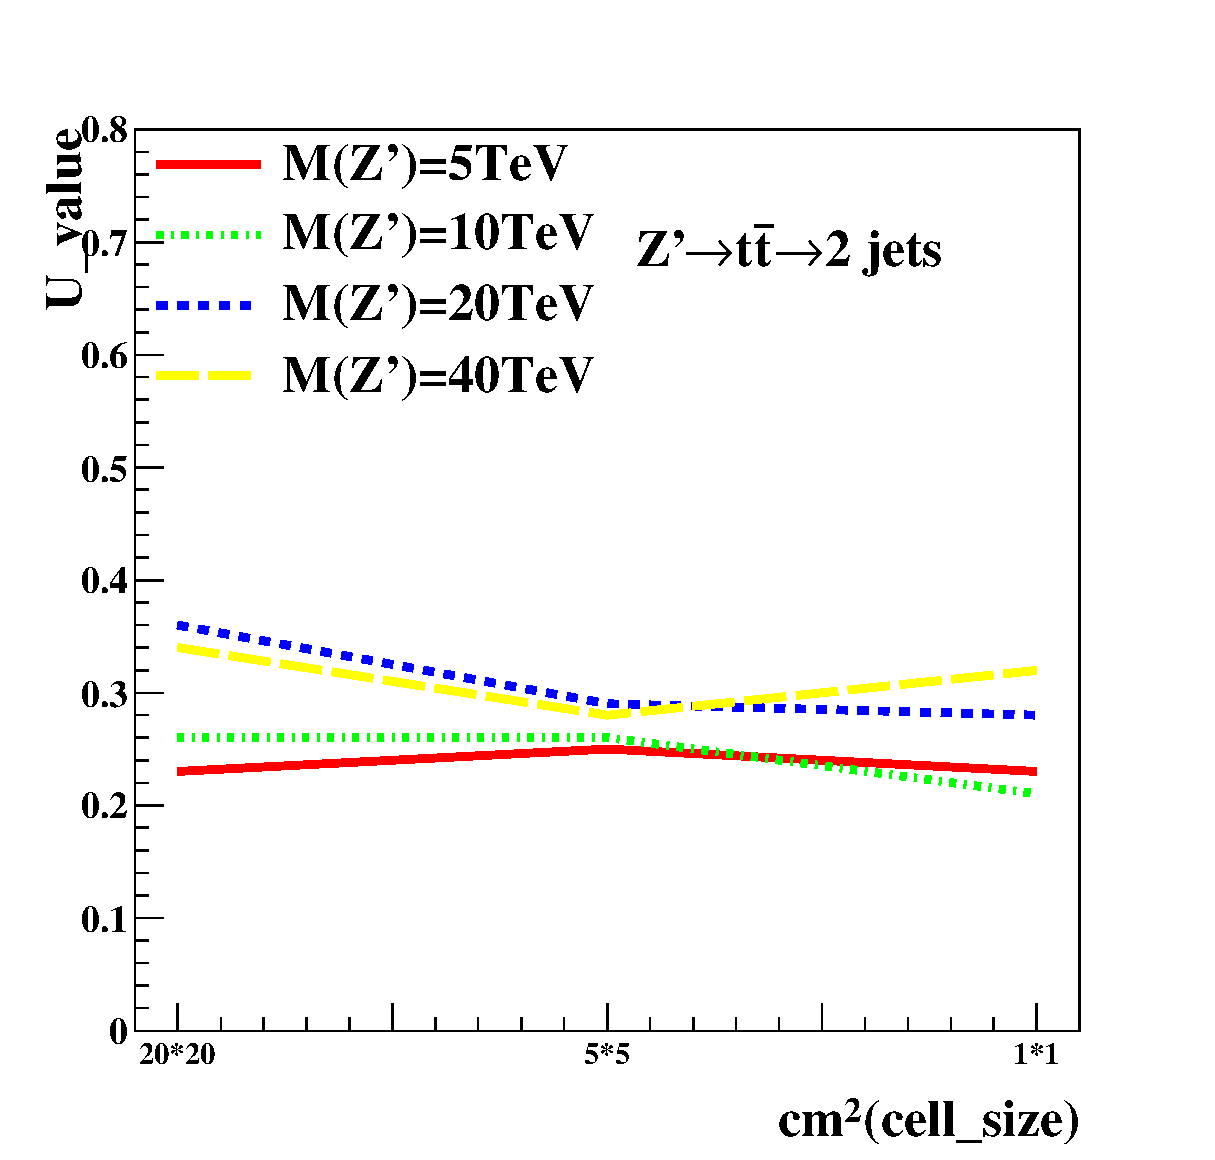
\includegraphics[width=0.3\textwidth]{Mann_Sum/raw_05_tau32_summary_U_after_cut_25bins_no_UOF_new_75pa.eps}
   }
   \subfigure[$C_2^{(1)}$] {
   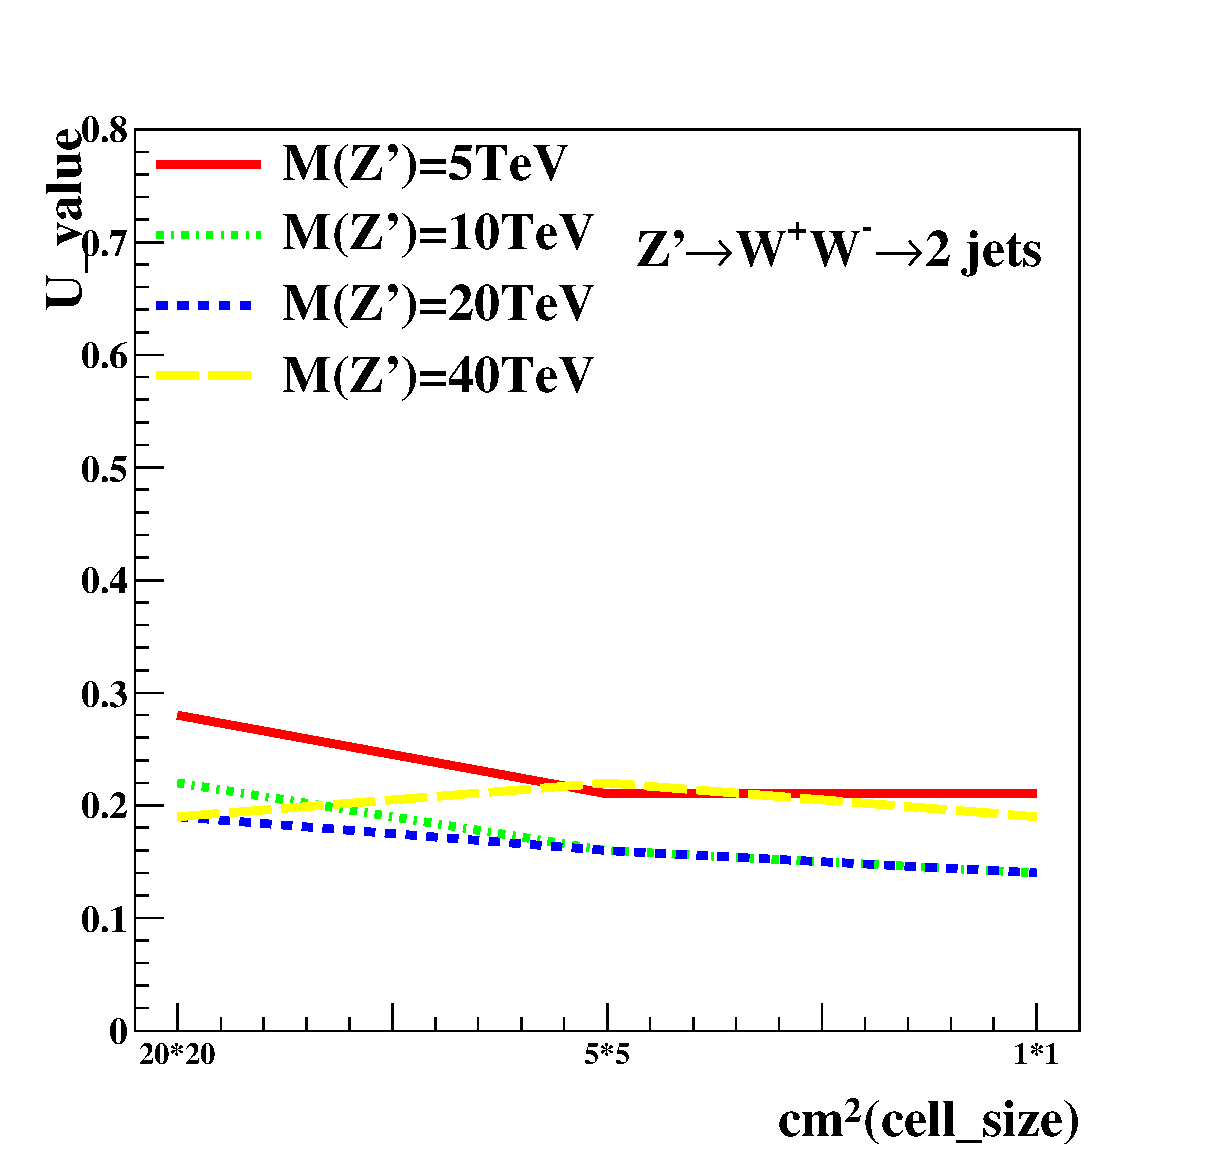
\includegraphics[width=0.3\textwidth]{Mann_Sum/raw_05_c2b1_summary_U_after_cut_25bins_no_UOF_new_75pa.eps}
   }
   \end{center}
\caption{The Mann-Whitney $U$ values for $\tau_{21}$, $\tau_{32}$, and $C_2^{(1)}$ 
reconstructed for different resonance masses and detector cell sizes. }
\label{fig:Rawhit_05GeV_total_Mann}
\end{figure}
\end{comment}
